\sgaStableTarget{sga6.e03.expose}\section*{第 III 讲. 相对有限性条件}
\begin{center}
L. Illusie
\end{center}

\sgaStableTarget{sga6.e03.sec.1}\section*{1. 相对伪凝聚性}

\sgaStableTarget{sga6.e03.thm.1-1}\textbf{定理 1.1.} 设 \(n\in \mathbb Z\). 对每个概形的局部有限型态射
\[
  f:X\longrightarrow Y
\]
存在唯一的 \(D(X)\)\footnote{\(D(X)\) 为 \(\mathcal O_X\)-模范畴的导出范畴.} 的满子范畴 \(D(f)_{n\text{-}\coh}\), 满足下列条件:

\begin{enumerate}[label=(\roman*)]
\item 若 \(E\in \Ob D(f)_{n\text{-}\coh}\), 则对每个开浸入 \(i:U\to X\), 有 \(i^*(E)\in \Ob D(fi)_{n\text{-}\coh}\).

\item 若 \(E\in \Ob D(X)\), 且存在开覆盖 \((i_\alpha:U_\alpha\to X)_{\alpha\in A}\), 使得对每个 \(\alpha\in A\) 都有 \(i_\alpha^*(E)\in \Ob D(fi_\alpha)_{n\text{-}\coh}\), 则 \(E\in \Ob D(f)_{n\text{-}\coh}\).

\item 若
\[
\begin{tikzcd}
X \arrow[r,"f"] \arrow[dr,"h"'] & Y \arrow[d,"g"]\\
& Z
\end{tikzcd}
\]
是局部有限型态射的交换三角形, 其中 \(f\) 为闭浸入, \(g\) 光滑, 则有
\[
  E\in \Ob D(h)_{n\text{-}\coh}
  \quad\Longleftrightarrow\quad
  f_*(E)\in D(Y)_{n\text{-}\coh}.
\]\footnote{\(D(Y)_{n\text{-}\coh}\) 为 \(D(Y)\) 中由 \(n\)-伪凝聚对象组成的满子范畴（\hyperlink{sga6.e01.ex.2-15}{I 2.15}）.}
\end{enumerate}

\emph{证明.} 唯一性是显然的. 事实上, 设 \(f:X\to Y\) 为局部有限型态射. 选取开覆盖 \((i_\alpha:X_\alpha\to X)_{\alpha\in A}\), 使得对每个 \(\alpha\), \(fi_\alpha\) 分解为
\[
  X_\alpha \xrightarrow{i'_\alpha} Y_\alpha \xrightarrow{f'_\alpha} Y,
\]
其中 \(i'_\alpha\) 为闭浸入, \(f'_\alpha\) 光滑. 由 (i)、(ii)、(iii) 立即可知, \(D(f)_{n\text{-}\coh}\) 的对象恰为满足
\[
  i'_{\alpha *}i_\alpha^*(E)\in \Ob D(Y_\alpha)_{n\text{-}\coh}
\]
的对象 \(E\in D(X)\); 因而作为 \(D(X)\) 的满子范畴, \(D(f)_{n\text{-}\coh}\) 被唯一确定. 为证明存在性, 需要几个引理.

\sgaStableTarget{sga6.e03.lem.1-1-1}\textbf{引理 1.1.1.} 设 \(i:X\to Y\) 为概形的闭浸入, 使得 \(i_*(\mathcal O_X)\) 伪凝聚, 并设 \(E\in \Ob D(X)\). \(E\) 为 \(n\)-伪凝聚的充要条件是 \(i_*(E)\) 为 \(n\)-伪凝聚的.

\emph{证明.} 必要性由伪凝聚性在应用函子下稳定的一般判据（\hyperlink{sga6.e01.prop.2-13}{I 2.13}）得出. 反之, 假设 \(i_*(E)\) 为 \(n\)-伪凝聚的, 下面证明 \(E\) 也如此. 由于 \(i_*(E)\) 的上同调局部上有界, \(E\) 的上同调也如此. 问题局部, 可以假设对充分大的 \(m\), \(E\) 为 \(m\)-伪凝聚的. 对 \(m\) 作递降归纳, 证明对每个 \(m\geq n\), \(E\) 均为 \(m\)-伪凝聚的. 可假设已证 \(E\) 为 \((n+1)\)-伪凝聚的. 局部化后, 存在特殊三角形
\[
\begin{tikzcd}[column sep=small,row sep=small]
&E''\arrow[dl]&\\
E'\arrow[rr]&&E\arrow[ul]
\end{tikzcd}
\]
其中 \(E'\) 完美, 且当 \(i>n\) 时 \(E''{}^i=0\). 由\hyperlink{sga6.e01.schol.2-6}{第 I 讲, 综合命题 2.6}, 只须证明 \(E''\) 为 \(n\)-伪凝聚的. 对上面的三角形应用 \(i_*\), 得到特殊三角形
\[
\begin{tikzcd}[column sep=small,row sep=small]
&i_*(E'')\arrow[dl]&\\
i_*(E')\arrow[rr]&&i_*(E)\arrow[ul]
\end{tikzcd}
\]
由证明的前半部分, \(i_*(E')\) 伪凝聚. 因而再由\hyperlink{sga6.e01.schol.2-6}{第 I 讲, 综合命题 2.6}, \(i_*(E'')\) 为 \(n\)-伪凝聚的. 由于 \(i_*(E'')\) 在次数 \(>n\) 时为零, 由\hyperlink{sga6.e01.prop.2-10}{第 I 讲, 命题 2.10} b), 这就是说 \(H^n(i_*(E''))\) 有限型. 但
\[
  H^n(i_*(E''))=i_*H^n(E''),
\]
因而再由\hyperlink{sga6.e01.prop.2-10}{第 I 讲, 命题 2.10} b), 断言归结为证明: 若 \(M\) 为 \(\mathcal O_X\)-模, 且 \(i_*(M)\) 有限型, 则 \(M\) 有限型. 这是直接的, 且不依赖于关于 \(i_*(\mathcal O_X)\) 的假设.

\sgaStableTarget{sga6.e03.rem.1-1-2}\textbf{注 1.1.2.} 上述引理特别适用于 \(i\) 为正则浸入（\hyperlink{sga6.e07.def.1-4}{VII 1.4}）的情形. 事实上, 借助 Koszul 复形, \(i_*(\mathcal O_X)\) 局部有一个由有限型自由 \(\mathcal O_Y\)-模组成的有限左消解; 因而 \(i_*(\mathcal O_X)\) 完美（\hyperlink{sga6.e01.ex.4-8}{I 4.8} 及 \hyperlink{sga6.e01.cor.4-14}{4.14}）, 从而更是伪凝聚的.

\sgaStableTarget{sga6.e03.lem.1-1-3}\textbf{引理 1.1.3.} 设
\[
\begin{tikzcd}
X' \arrow[r,"f"] \arrow[d,"i'"'] & X \arrow[d,"i"]\\
Y' \arrow[r,"g"'] & Y
\end{tikzcd}
\]
为概形的笛卡尔方块, 其中 \(i\) 为闭浸入, 并设 \(E\) 为 \(\mathcal O_X\)-模复形. 则:
\begin{enumerate}[label=(\roman*)]
\item 典范基变换箭头（EGA III 1.4.15.4）
\[
  g^*i_*(E)\longrightarrow i'_*f^*(E)
\]
为同构.

\item 令 \(E'=f^*(E)\). 若 \(g\) 平坦, 且 \(i_*(E)\) 为 \(n\)-伪凝聚的, 则 \(i'_*(E')\) 为 \(n\)-伪凝聚的. 反之, 若 \(g\) 忠实平坦, 且 \(i'_*(E')\) 为 \(n\)-伪凝聚的, 则 \(i_*(E)\) 为 \(n\)-伪凝聚的.
\end{enumerate}

\emph{证明.} 在各点的茎上平凡地验证即可.

\sgaStableTarget{sga6.e03.lem.1-1-4}\textbf{引理 1.1.4.} 设
\[
\begin{tikzcd}
X' \arrow[dr,"f'"'] & X \arrow[l,"i'"'] \arrow[r,"i''"] & X''\arrow[dl,"f''"]\\
& Y &
\end{tikzcd}
\]
为概形的交换图, 其中 \(i'\), 分别为 \(i''\), 为闭浸入, \(f'\), 分别为 \(f''\), 光滑, 且 \(E\in \Ob D(X)\). 则
\[
  i'_*(E)\text{ 为 }n\text{-伪凝聚的}
  \quad\Longleftrightarrow\quad
  i''_*(E)\text{ 为 }n\text{-伪凝聚的}.
\]

\emph{证明.} 使用 Lichtenbaum 的一个技巧, 将 \(X\) 对角地映入 \(X'\times_YX''\). 立即可归结为证明 \(f'\)、\(f''\) 之一为恒等映射时的断言. 更改记号, 得到交换三角形
\[
\begin{tikzcd}
& Y \arrow[d,"f"]\\
X \arrow[r,"j"'] \arrow[ur,"i"] & Z
\end{tikzcd}
\]
其中 \(i\) 和 \(j\) 为闭浸入, \(f\) 光滑; 需要证明 \(i_*(E)\) 为 \(n\)-伪凝聚的, 当且仅当 \(j_*(E)\) 为 \(n\)-伪凝聚的. 问题在 \(Y\) 和 \(Z\) 上的 \(X\) 中某点的邻域中局部, 故可假设 \(X,Y,Z\) 均仿射, 且有分解
\[
\begin{tikzcd}
Y \arrow[r,"i'"] \arrow[d,"f"'] & Z[T_1,\ldots,T_r]\arrow[dl,"f'"]\\
Z&
\end{tikzcd}
\]
其中 \(i'\) 为闭浸入, 斜箭头为典范投影. 由\hyperlink{sga6.e07.prop.1-10}{第 VII 讲, 1.10}, \(i'\) 为正则浸入; 因而由\hyperlink{sga6.e03.lem.1-1-1}{引理 1.1.1}, \(D(Y)\) 的对象 \(F\) 为 \(n\)-伪凝聚的, 当且仅当 \(i'_*(F)\) 为 \(n\)-伪凝聚的.

因而可假设 \(Y=Z[T_1,\ldots,T_r]\), \(f\) 为典范投影. 图 \((*)\) 便对应于环图
\[
\begin{tikzcd}
& B=C[T_1,\ldots,T_r]\arrow[dl,"u"']\\ A & C\arrow[l,"v"]\arrow[u,"c"']
\end{tikzcd}
\]
其中 \(u\) 和 \(v\) 为满射, \(c:C\to B\) 为典范包含映射. 对 \(1\leq i\leq r\), 令 \(u(T_i)=x_i\), 并取 \(z_i\in C\) 使 \(v(z_i)=x_i\). 由
\[
  \sigma:B\longrightarrow C,\qquad \sigma(T_i)=z_i,
\]
定义的 \(c\) 的收缩 \(\sigma\) 满足 \(v\sigma=u\). 用几何语言说, 它对应于 \(f\) 的一个截面 \(s\), 满足 \(i=sj\). 由\hyperlink{sga6.e07.prop.1-10}{第 VII 讲, 1.10}, \(s\) 为正则浸入; 于是断言由\hyperlink{sga6.e03.lem.1-1-1}{引理 1.1.1} 得出.

\emph{\hyperlink{sga6.e03.thm.1-1}{定理 1.1} 的证明（续完）.} 设 \(f:X\to Y\) 为局部有限型态射. 存在 \(X\) 的开覆盖 \((X_\alpha)\), 使每个 \(X_\alpha\) 都可闭浸入 $Y$ 上光滑的某个概形 \(Y_\alpha\). 令 \(\coprod X_\alpha=X'\), \(\coprod Y_\alpha=Y'\). 有交换图
\[
\begin{tikzcd}
X' \arrow[r,"i'"] \arrow[d,"p'"'] & Y' \arrow[ddl,"f'"]\\
X \arrow[d,"f"']\\
Y
\end{tikzcd}\tag{a'}
\]
其中 \(p'\) 为满射开浸入族的和（为简便起见, 称其为\emph{特殊态射（special）}）, \(i'\) 为闭浸入, \(f'\) 光滑. 将 \(D(f)_{n\text{-}\coh}\) 定义为 \(D(X)\) 中由使 \(i'_*p'{}^*(E)\) 为 \(n\)-伪凝聚的对象 \(E\) 组成的满子范畴. 首先证明这一定义有意义, 即 \(D(f)_{n\text{-}\coh}\) 与 \(i'\)、\(p'\)、\(f'\) 的选择无关. 设
\[
\begin{tikzcd}
X'' \arrow[r,"i''"] \arrow[d,"p''"'] & Y'' \arrow[ddl,"f''"]\\
X \arrow[d,"f"']\\
Y
\end{tikzcd}\tag{a''}
\]
为类似于 \((a')\) 的交换图, 其中 \(p''\) 为特殊态射, \(i''\) 为闭浸入, \(f''\) 光滑. 由 \((a')\) 与 \((a'')\) 得到交换图
\[
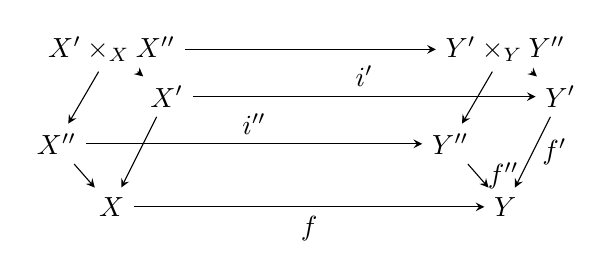
\begin{tikzpicture}[>=stealth,baseline=(current bounding box.center)]
\node (A) at (0,2) {$X'\times_X X''$};\node (B) at (-.7,.8) {$X''$};\node (C) at (.7,1.4) {$X'$};\node (D) at (0,0) {$X$};
\node (E) at (5,2) {$Y'\times_Y Y''$};\node (F) at (4.3,.8) {$Y''$};\node (G) at (5.7,1.4) {$Y'$};\node (H) at (5,0) {$Y$};
\draw[->] (A)--(B);\draw[->] (A)--(C);\draw[->] (B)--(D);\draw[->] (C)--(D);\draw[->] (E)--(F);\draw[->] (E)--(G);\draw[->] (F)--node[right]{$f''$}(H);\draw[->] (G)--node[right]{$f'$}(H);
\draw[->] (A)--(E);\draw[->] (B)--node[above]{$i''$}(F);\draw[->] (C)--node[above]{$i'$}(G);\draw[->] (D)--node[below]{$f$}(H);
\end{tikzpicture}
\]
其中除 \(f\) 外的水平箭头均为闭浸入, 左侧, 分别右侧, 的笛卡尔方块中的箭头均为特殊态射, 分别为光滑态射. 因而归结为证明下述断言.

\textbf{(A)} 设
\[
\begin{tikzcd}
X_1 \arrow[r,"i_1"] \arrow[d,"p"'] & Y_1 \arrow[d,"q"]\\
X_2 \arrow[r,"i_2"'] & Y_2
\end{tikzcd}
\]
为概形的交换方块, 其中 \(p\) 为特殊态射, \(q\) 光滑, \(i_1\)、\(i_2\) 为闭浸入, 且 \(E\in \Ob D(X_2)\). 则 \(i_{2*}(E)\) 为 \(n\)-伪凝聚的, 当且仅当 \(i_{1*}p^*(E)\) 为 \(n\)-伪凝聚的.

\emph{该断言的证明.} 按定义, \(p\) 为覆盖 \(X_2\) 的一族开集 \(U_\alpha\) 之和. 每个 \(U_\alpha\) 都由 \(Y_2\) 的一个开集 \(V_\alpha\) 诱导, 各个 \(V_\alpha\) 覆盖 \(X_2\) 在 \(Y_2\) 中的一个开邻域 \(X'_2\). 因此有笛卡尔交换图
\[
\begin{tikzcd}
X_1 \arrow[r,"i'_1"] \arrow[d,"p"'] & X'_1 \arrow[d,"p'"]\\
X_2 \arrow[r,"i'_2"'] \arrow[rr,"i_2"',bend right=25] & X'_2 \arrow[r,"j"'] & Y_2
\end{tikzcd}
\]
其中 \(i'_1\)、\(i'_2\) 为闭浸入, \(p\)、\(p'\) 为特殊态射, \(j\) 为开浸入. 条件 \(i_{2*}(E)\) 为 \(n\)-伪凝聚的, 显然等价于条件 \(i'_{2*}(E)\) 为 \(n\)-伪凝聚的. 另一方面, 由\hyperlink{sga6.e03.lem.1-1-3}{引理 1.1.3}, 条件 \(i'_{2*}(E)\) 为 \(n\)-伪凝聚的, 等价于条件 \(i'_{1*}p^*(E)\) 为 \(n\)-伪凝聚的. 最后对 \(i_2p\) 的两个分解 \((jp')i'_1\) 与 \(qi_1\), 以及 \(p^*(E)\in \Ob D(X_1)\) 应用\hyperlink{sga6.e03.lem.1-1-4}{引理 1.1.4}, 即知 \(i_{2*}(E)\) 为 \(n\)-伪凝聚的, 当且仅当 \(i_{1*}p^*(E)\) 为 \(n\)-伪凝聚的, 正如所需.

由此已证, 通过图 \((a')\) 定义的范畴 \(D(f)_{n\text{-}\coh}\) 实际上只依赖于 \(f\). 此外, 由定义可平凡地看出它满足 (i) 至 (iii). \hyperlink{sga6.e03.thm.1-1}{定理 1.1} 得证.

\sgaStableTarget{sga6.e03.def.1-2}\textbf{定义 1.2.} 设 \(f:X\to Y\) 为局部有限型态射, \(E\in \Ob D(X)\), \(n\in\mathbb Z\). 若 \(E\in \Ob D(f)_{n\text{-}\coh}\)（参见 \hyperlink{sga6.e03.thm.1-1}{1.1}）, 则称 \(E\) 关于 \(f\) 为 \(n\)-伪凝聚的. 若对每个 \(n\in\mathbb Z\), \(E\) 关于 \(f\) 都为 \(n\)-伪凝聚的, 则称 \(E\) 关于 \(f\) 伪凝聚, 或 \((-\infty)\)-伪凝聚. 以 \(D(f)_{\mathrm{coh}}\) 表示 \(D(X)\) 中由关于 \(f\) 伪凝聚的对象组成的满子范畴.

若 \(\mathcal O_X\) 关于 \(f\) 为 \(n\)-伪凝聚的, 分别为伪凝聚的, 则称 \(f\) 为 \(n\)-伪凝聚的, 分别为伪凝聚的. 在不会引起混淆时, 有时用“关于 \(Y\) 为 \(n\)-伪凝聚的, 分别为伪凝聚的”代替“关于 \(f\)”, 并用
\[
  D(X)_{Y,n\text{-}\coh}\quad(\text{分别为 }D(X)_{Y,\coh})
\]
代替
\[
  D(f)_{n\text{-}\coh}\quad(\text{分别为 }D(f)_{\mathrm{coh}}).
\]
最后, 对 \(*=+,-,b\), 令
\[
  D^*(f)_{n\text{-}\coh}=D^*(X)\cap D(f)_{n\text{-}\coh},
  \qquad
  D^*(f)_{\mathrm{coh}}=D^*(X)\cap D(f)_{\mathrm{coh}}.
\]

\sgaStableTarget{sga6.e03.rem.1-2-1}\textbf{注 1.2.1.}
\begin{enumerate}[label=\alph*)]
\item 范畴 \(D(f)_{n\text{-}\coh}\)、\(D(f)_{\mathrm{coh}}\) 一般不包含在 \(D^{-}(X)\) 中. 但当 \(X\) 拟紧时包含, 因为此时 \(D(X)\) 中上同调局部上有界的对象的上同调上有界.

\item \(D(f)_{\mathrm{coh}}\) 的对象的上同调拟凝聚. 事实上, 若 \(E\in \Ob D(f)_{\mathrm{coh}}\), 问题局部, 故可假设 \(f\) 为闭浸入; 于是 \(f_*(E)\) 伪凝聚, 因而其上同调拟凝聚, 再利用下述事实: \(\mathcal O_X\)-模 \(M\) 拟凝聚当且仅当 \(f_*(M)\) 拟凝聚.

\item 对 \(\mathcal O_X\)-模, 将使用“关于 \(f\) 有限表现”的术语, 而不用“关于 \(f\) 为 \((-1)\)-伪凝聚的”. 由\hyperlink{sga6.e01.prop.2-9}{第 I 讲, 命题 2.9}, \(\mathcal O_X\)-模 \(E\) 关于 \(f\) 有限表现的充要条件是: 局部存在闭浸入 \(i:X\to X'\), 其中 \(X'\) 在 \(Y\) 上光滑, 使得 \(i_*(E)\) 在通常意义下有限表现. 特别地, 说 \(f\) 为 \((-1)\)-伪凝聚的, 等价于说 \(f\) 在 EGA IV 1.4 的意义下局部有限表现.
\end{enumerate}

\sgaStableTarget{sga6.e03.ex.1-3}\textbf{例 1.3.} 光滑态射及正则浸入（\hyperlink{sga6.e03.rem.1-1-2}{1.1.2}）都是伪凝聚态射. 若 \(Y\) 局部诺特, 则任意局部有限型态射 \(f:X\to Y\) 都是伪凝聚态射.

\sgaStableTarget{sga6.e03.prop.1-4}\textbf{命题 1.4.} 设 \(f:X\to Y\) 为局部有限型态射, 并设
\[
\begin{tikzcd}[column sep=small,row sep=small]
&G\arrow[dl]&\\
E\arrow[rr]&&F\arrow[ul]
\end{tikzcd}
\]
为 \(D(X)\) 的特殊三角形. 在下表中, \(n\in \mathbb Z\cup\{-\infty\}\) 表示关于 \(f\) 的伪凝聚性的次数; 每一行代表一个蕴含关系, 其中结论加下划线:
\[
\begin{array}{ccc}
E&F&G\\
n+1&n&\underline n\\
n&\underline n&n\\
\underline n&n&n-1.
\end{array}
\]
特别地, \(D(f)_{\mathrm{coh}}\) 是 \(D(X)\) 的三角子范畴.

\emph{证明.} 由\hyperlink{sga6.e03.thm.1-1}{定理 1.1} 的性质 (i) 至 (iii), 可假设 \(f\) 为闭浸入. 于是有特殊三角形
\[
\begin{tikzcd}[column sep=small,row sep=small]
&f_*(G)\arrow[dl]&\\
f_*(E)\arrow[rr]&&f_*(F)\arrow[ul]
\end{tikzcd}
\]
断言便由\hyperlink{sga6.e01.schol.2-6}{第 I 讲, 综合命题 2.6} 得出.

\sgaStableTarget{sga6.e03.def.1-5}\textbf{定义 1.5.} 设 \(X,Y\) 为两个 \(S\)-概形. 若
\[
  \Tor_i^S(\mathcal O_X,\mathcal O_Y)=0\quad\text{当 }i\ne 0,
\]
则称 \(X,Y\) \emph{在 \(S\) 上 Tor-无关（Tor-independent）}, 其中 \(\Tor_i^S\) 为 EGA III 6.5 中定义的局部超 Tor 层. 这是一个局部性质. 若 \(X,Y,S\) 仿射, 相应的环为 \(B,C,A\), 则此条件意为典范映射
\[
  B\otimes_A^{\mathbf L}C\longrightarrow B\otimes_A C
\]
为同构. 因而若 \(X\) 或 \(Y\) 在 \(S\) 上平坦, 此条件特别地满足.

\sgaStableTarget{sga6.e03.lem.1-5-1}\textbf{引理 1.5.1.} 设
\[
\begin{tikzcd}
X \arrow[d] & X' \arrow[l] \arrow[d] & X'' \arrow[l] \arrow[d]\\
Y & Y' \arrow[l] & Y'' \arrow[l]
\end{tikzcd}
\]
为概形的笛卡尔方块. 若 \(X\) 与 \(Y'\) 在 \(Y\) 上 Tor-无关, 且 \(X'\) 与 \(Y''\) 在 \(Y'\) 上 Tor-无关, 则 \(X\) 与 \(Y''\) 在 \(Y\) 上 Tor-无关.

\emph{证明.} 这是关于张量积结合性的简单练习.

\sgaStableTarget{sga6.e03.notation.1-6}\textbf{记号 1.6.} 设 \(X,Y\) 为两个 \(S\)-概形, \(E\in \Ob D^{-}(X)\), \(F\in \Ob D^{-}(Y)\). 令
\[
  E\otimes_S^{\mathbf L}F
  =
  L\pr_1^*(E)\otimes^{\mathbf L}L\pr_2^*(F),
\]
其中 \(\pr_1,\pr_2\) 为 \(X\times_SY\) 的两个投影.

\sgaStableTarget{sga6.e03.lem.1-7}\textbf{引理 1.7.} 设 \(S\) 为概形, 并对 \(i=1,2\) 设
\[
  f_i:X_i\longrightarrow Y_i
\]
为闭 \(S\)-浸入. 假设 \(X_1\) 与 \(X_2\), 以及 \(Y_1\) 与 \(Y_2\), 都在 \(S\) 上 Tor-无关. 则对 \(E_i\in \Ob D^{-}(X_i)_{\mathrm{qcoh}}\),\footnote{\(D(X_i)_{\qcoh}\) 表示 \(D(X_i)\) 中由上同调拟凝聚的复形组成的满子范畴.} 有典范同构
\[
  f_{1*}(E_1)\otimes_S^{\mathbf L} f_{2*}(E_2)
  \xrightarrow{\sim}
  (f_1\times_S f_2)_*(E_1\otimes_S^{\mathbf L}E_2).
\]

\emph{证明.} 令 \(f_1\times_Sf_2=f\). 由伴随性容易定义典范箭头
\[
  f_{1*}(E_1)\otimes_S^{\mathbf L} f_{2*}(E_2)
  \longrightarrow
  f_*(E_1\otimes_S^{\mathbf L}E_2).
\]
下面证明它是同构. 问题局部, 可假设 \(S,X_i,Y_i\) 仿射, 相应的环为 \(C,A_i,B_i\). 经逐步分解, 可归结为 \(E_i=\mathcal O_{X_i}\). 此时须验证
\[
  A_1\otimes^{\mathbf L}_{B_1}B\otimes^{\mathbf L}_{B_2}A_2
  \longrightarrow A
\]
为同构, 其中 \(A=A_1\otimes_C A_2\), \(B=B_1\otimes_C B_2\). 由 Tor-无关的假设及张量积的结合性, 这立即得出.

\sgaStableTarget{sga6.e03.prop.1-8}\textbf{命题 1.8.} 设 \(S\) 为概形, 并对 \(i=1,2\) 设
\[
  f_i:X_i\longrightarrow Y_i
\]
为局部有限型 \(S\)-态射. 假设 \(X_1\) 与 \(X_2\), 以及 \(Y_1\) 与 \(Y_2\), 都在 \(S\) 上 Tor-无关. 设 \([a_i,b_i]\) 为 \(\mathbb Z\) 的区间, 并设
\[
  E_i\in \Ob D^{-}(X_i)_{\mathrm{qcoh}}
\]
是关于 \(f_i\) 为 \(a_i\)-伪凝聚, 且在次数 \(>b_i\) 时无上同调的复形. 则
\[
  E_1\otimes_S^{\mathbf L}E_2
\]
关于 \(f=f_1\times_S f_2\) 为 \(a\)-伪凝聚的, 且在次数 \(>b\) 时无上同调, 其中
\[
  a=\sup(a_1+b_2,a_2+b_1),\qquad b=b_1+b_2.
\]

\emph{证明.} 问题在 \(X_1\times_SX_2\) 上局部, 可假设 \(f_i\) 分解为
\[
  X_i\xrightarrow{f'_i}Y'_i\xrightarrow{p_i}Y_i,
\]
其中 \(f'_i\) 为闭浸入, \(p_i\) 为光滑态射. 令 \(f'=f'_1\times_Sf'_2\). 需要证明 \(f'_*(E_1\otimes_S^{\mathbf L}E_2)\) 为 \(a\)-伪凝聚的, 且在次数 \(>b\) 时无上同调. 由\hyperlink{sga6.e03.lem.1-5-1}{引理 1.5.1}, \(Y'_1\) 与 \(Y'_2\) 在 \(S\) 上 Tor-无关. 更改记号后, 可假设 \(f_i=f'_i\), 即各个 \(f_i\) 为闭浸入. 由假设, \(f_{i*}(E_i)\) 为 \(a_i\)-伪凝聚的, 且在次数 \(>b_i\) 时无上同调; 因而由\hyperlink{sga6.e01.cor.2-16}{第 I 讲, 推论 2.16},
\[
  f_{1*}(E_1)\otimes_S^{\mathbf L}f_{2*}(E_2)
\]
为 \(a\)-伪凝聚的, 且在次数 \(>b\) 时无上同调. 再用\hyperlink{sga6.e03.lem.1-7}{引理 1.7} 便得结论.

\sgaStableTarget{sga6.e03.cor.1-9}\textbf{推论 1.9.} 在\hyperlink{sga6.e03.prop.1-8}{命题 1.8} 的假设下, 函子
\[
  \otimes_S^{\mathbf L}:D^{-}(X_1)\times D^{-}(X_2)\longrightarrow D^{-}(X)
\]
诱导函子
\[
  \otimes_S^{\mathbf L}:D^{-}(f_1)_{\mathrm{coh}}\times D^{-}(f_2)_{\mathrm{coh}}
  \longrightarrow D^{-}(f)_{\mathrm{coh}} .
\]
特别地, 若 \(f_1\) 和 \(f_2\) 伪凝聚, 则 \(f\) 也伪凝聚.

\sgaStableTarget{sga6.e03.cor.1-10}\textbf{推论 1.10.} 设
\[
\begin{tikzcd}
X' \arrow[r,"g"] \arrow[d,"f'"'] & X \arrow[d,"f"]\\
Y' \arrow[r,"h"'] & Y
\end{tikzcd}
\]
为笛卡尔方块, 其中 \(f\) 局部有限型. 则:
\begin{enumerate}[label=\alph*)]
\item 假设 \(X\) 与 \(Y'\) 在 \(Y\) 上 Tor-无关. 对 \(n\in\mathbb Z\cup\{-\infty\}\), 函子 \(Lg^*:D^{-}(X)\to D^{-}(X')\) 诱导函子
\[
  Lg^*:D^{-}(f)_{n\text{-}\coh}\longrightarrow D^{-}(f')_{n\text{-}\coh}.
\]
特别地, 若 \(f\) 为 \(n\)-伪凝聚的, 则 \(f'\) 也为 \(n\)-伪凝聚的.

\item 假设 \(h\) 忠实平坦. 设 \(n\in\mathbb Z\cup\{-\infty\}\), \(E\in\Ob D^{-}(X)\) 为上同调拟凝聚的复形. \(E\) 关于 \(f\) 为 \(n\)-伪凝聚的充要条件是 \(g^*(E)\) 关于 \(f'\) 为 \(n\)-伪凝聚的. 特别地, \(f\) 为 \(n\)-伪凝聚的充要条件是 \(f'\) 为 \(n\)-伪凝聚的.
\end{enumerate}

\emph{证明.} 考虑到\hyperlink{sga6.e03.rem.1-2-1}{注 1.2.1} b), 推论 \hyperlink{sga6.e03.cor.1-9}{1.9} 和 \hyperlink{sga6.e03.cor.1-10}{1.10} 的所有断言都平凡地由\hyperlink{sga6.e03.prop.1-8}{命题 1.8} 得出, 唯一例外是 \hyperlink{sga6.e03.cor.1-10}{1.10} b) 的充分性. 对此, 问题在 \(X\) 上局部, 可假设 \(f\) 分解为闭浸入后接光滑态射. 由\hyperlink{sga6.e03.lem.1-1-3}{引理 1.1.3}, 归结为 \(f\), 分别为 \(f'\), 是 \(X\), 分别为 \(X'\), 的恒等映射的情形. 由标准的逐步分解论证（参见 \hyperlink{sga6.e01.exercise.2-16-2}{I 2.16.2}）, 断言便来自下述事实: \(X\) 上的拟凝聚层 \(L\) 有限型当且仅当 \(g^*L\) 有限型.

\sgaStableTarget{sga6.e03.prop.1-11}\textbf{命题 1.11.} 设
\[
\begin{tikzcd}
X \arrow[r,"f"] \arrow[dr,"h"'] & Y \arrow[d,"g"]\\
& Z
\end{tikzcd}
\]
为局部有限型态射的交换三角形. 设 \(E\in\Ob D(X)\), \(F\in\Ob D(Y)\), \([a,b]\)、\([c,d]\) 为 \(\mathbb Z\) 的区间.

\begin{enumerate}[label=\alph*)]
\item 若 \(E\) 关于 \(f\) 为 \(a\)-伪凝聚的, 且在次数 \(>b\) 时无上同调, 而 \(F\) 关于 \(g\) 为 \(c\)-伪凝聚的, 且在次数 \(>d\) 时无上同调, 则
\[
  E\otimes_{\mathcal O_Y}^{\mathbf L}F
\]
关于 \(h\) 为 \(m\)-伪凝聚的, 且在次数 \(>n\) 时无上同调, 其中
\[
  m=\sup(a+d,b+c),\qquad n=b+d.
\]

\item 若 \(E\) 关于 \(h\) 为 \(a\)-伪凝聚的, 且在次数 \(>b\) 时无上同调, 而 \(g\) 为 \((a+1-b)\)-伪凝聚的, 则 \(E\) 关于 \(f\) 为 \(a\)-伪凝聚的.
\end{enumerate}

\emph{证明.} 问题在 \(X\) 上局部, 可假设有笛卡尔交换图
\[
\begin{tikzcd}[column sep=small,row sep=small]
&& E^{r+s}_Z\arrow[dr] &&\\
& E^r_Y\arrow[ur,"j"]\arrow[dr,"p"] && E^s_Z\arrow[dr,"q"] &\\
X\arrow[ur,"i"]\arrow[rr,"f"'] && Y\arrow[ur,"k"]\arrow[rr,"g"'] && Z
\end{tikzcd}
\]
其中 \(i,j,k\) 为闭浸入, \(p,q\) 为仿射空间的典范投影. 若 \(F\) 关于 \(Z\) 为 \(c\)-伪凝聚的, 则由\hyperlink{sga6.e03.thm.1-1}{定理 1.1 (iii)}, \(k_*(F)\) 为 \(c\)-伪凝聚的, 再由\hyperlink{sga6.e03.lem.1-1-3}{引理 1.1.3}, \(j_*p^*(F)\) 为 \(c\)-伪凝聚的. 类似地, 若 \(g\) 为 \(x\)-伪凝聚的, 则 \(j_*(\mathcal O_{E^r_Y})\) 为 \(x\)-伪凝聚的. 因此由相对伪凝聚性的定义, 可归结为 \(f\) 与 \(g\) 都为闭浸入时证明 a)、b).

\emph{a) 的证明.} 由\hyperlink{sga6.e03.thm.1-1}{定理 1.1 (iii)}, 需要证明下述断言: 若 \(f_*(E)\) 为 \(a\)-伪凝聚的, 且在次数 \(>b\) 时无上同调, \(g_*(F)\) 为 \(c\)-伪凝聚的, 且在次数 \(>d\) 时无上同调, 则
\[
  h_*(E\otimes_Y^{\mathbf L}F)
\]
为 \(m\)-伪凝聚的, 且在次数 \(>n\) 时无上同调. 有典范同构
\[
  f_*(E)\otimes_Y^{\mathbf L}F\xrightarrow{\sim} f_*(E\otimes_Y^{\mathbf L}F),
\]
这是\hyperlink{sga6.e03.prop.1-8}{命题 1.8} 证明中使用的同构的特例. 由于函子 \(g_*(-\otimes^{\mathbf L}F)\) 将有限型局部自由层变成 \(c\)-伪凝聚复形, 并将次数 \(>0\) 时无上同调的复形变成次数 \(>d\) 时无上同调的复形, 断言便由\hyperlink{sga6.e01.prop.2-13}{第 I 讲, 命题 2.13} 得出.

\emph{b) 的证明.} 需要证明下述断言: 假设 \(f_*(E)\) 为 \(a\)-伪凝聚的, 且在次数 \(>b\) 时无上同调, 而 \(g_*(\mathcal O_Y)\) 为 \((a+1-b)\)-伪凝聚的. 则 \(f_*(E)\) 为 \(a\)-伪凝聚的. 由于断言只涉及 \(f_*(E)\), 可假设 \(X=Y\) 且 \(f=\Id_X\). 此后按\hyperlink{sga6.e03.lem.1-1-1}{引理 1.1.1} 的证明方法, 递降归纳证明 \(E\) 在所有次数 \(\geq a\) 伪凝聚. 假设已证 \(E\) 为 \((a+1)\)-伪凝聚的. 由\hyperlink{sga6.e01.prop.2-10}{第 I 讲, 命题 2.10}, 局部化后存在特殊三角形
\[
\begin{tikzcd}[column sep=small,row sep=small]
&E''\arrow[dl]&\\
E'\arrow[rr]&&E\arrow[ul]
\end{tikzcd}
\]
其中当 \(i\in [a+1,b]\) 时 \(E'{}^i\) 局部自由, 当 \(i\notin [a+1,b]\) 时 \(E'{}^i=0\), 当 \(i>a\) 时 \(E''{}^i=0\). 由 \(g_*(\mathcal O_Y)\) 为 \((a+1-b)\)-伪凝聚的假设及\hyperlink{sga6.e01.prop.2-11}{第 I 讲, 命题 2.11} a), \(g_*(E')\) 为 \((a+1)\)-伪凝聚的. 由于 \(g_*(E)\) 为 \(a\)-伪凝聚的, 由\hyperlink{sga6.e01.schol.2-6}{第 I 讲, 综合命题 2.6}, \(g_*(E'')\) 为 \(a\)-伪凝聚的. 再用\hyperlink{sga6.e01.prop.2-10}{第 I 讲, 命题 2.10} b), 以及 \(\mathcal O_Y\)-模 \(M\) 有限型当且仅当 \(g_*(M)\) 有限型这一事实, 便得结论. 推论 \hyperlink{sga6.e03.cor.1-12}{1.12}--\hyperlink{sga6.e03.cor.1-14}{1.14} 立即得出.

\sgaStableTarget{sga6.e03.cor.1-12}\textbf{推论 1.12.} 在\hyperlink{sga6.e03.prop.1-11}{命题 1.11} 的情形中, 若 \(g\) 伪凝聚, 则对 \(r\in\mathbb Z\cup\{-\infty\}\),
\[
  D^{-}(f)_{r\text{-}\coh}=D^{-}(h)_{r\text{-}\coh}.
\]
特别地, 取 \(X=Y\), 则 \(Y\) 上绝对意义下的 \(r\)-伪凝聚性与关于 \(g\) 的 \(r\)-伪凝聚性一致.

\sgaStableTarget{sga6.e03.cor.1-13}\textbf{推论 1.13.} 在\hyperlink{sga6.e03.prop.1-11}{命题 1.11} 的情形中, 若 \(f\) 伪凝聚, 则函子
\[
  \mathcal O_X\otimes_Y^{\mathbf L}-=Lf^*:D^{-}(Y)\longrightarrow D^{-}(X)
\]
对 \(r\in\mathbb Z\cup\{-\infty\}\) 诱导函子
\[
  Lf^*:D^{-}(g)_{r\text{-}\coh}\longrightarrow D^{-}(h)_{r\text{-}\coh}.
\]

\sgaStableTarget{sga6.e03.cor.1-14}\textbf{推论 1.14.} 在\hyperlink{sga6.e03.prop.1-11}{命题 1.11} 的情形中, 若 \(f\) 为 \(r\)-伪凝聚的, \(g\) 为 \(s\)-伪凝聚的, 其中 \(r,s\in\mathbb Z\cup\{-\infty\}\), 则 \(h\) 为 \(\sup(r,s)\)-伪凝聚的. 若 \(h\) 为 \(r\)-伪凝聚的, \(g\) 为 \((r+1)\)-伪凝聚的, 则 \(f\) 为 \(r\)-伪凝聚的.

\sgaStableTarget{sga6.e03.rem.1-14-1}\textbf{注 1.14.1.} 特别地, 取 \(r=s=-1\), 得到（参见 \hyperlink{sga6.e03.rem.1-2-1}{1.2.1} c)）EGA IV 1.4.3 的断言 (ii)、(v).

\sgaStableTarget{sga6.e03.sec.2}\section*{2. 有限性定理}

\sgaStableTarget{sga6.e03.conj.2-1}\textbf{猜想 2.1.} 设 \(S\) 为概形, \(f:X\to Y\) 为 $S$ 上局部有限型概形之间的固有 \(S\)-态射, 且 \(E\in \Ob D^+(X)\). 若 \(E\) 关于 \(S\) 伪凝聚, 则 \(\mathbf R f_*(E)\) 也如此.

\sgaStableTarget{sga6.e03.thm.2-2}\textbf{定理 2.2.} 上述猜想在以下情形中成立:
\[
  \text{(i) } S\text{ 局部诺特};\qquad
  \text{(ii) } f\text{ 为射影态射}.
\]

\emph{情形 (i) 的证明.} 由于 \(S\) 局部诺特, \(X\), 分别为 \(Y\), 到 \(S\) 的投影为伪凝聚态射, 而 \(X\), 分别为 \(Y\), 上的伪凝聚性与关于 \(S\) 的伪凝聚性一致（\hyperlink{sga6.e03.cor.1-12}{推论 1.12}）. 另一方面, 由于 \(X\), 分别为 \(Y\), 局部诺特, 因而 \(\mathcal O_X\), 分别为 \(\mathcal O_Y\), 凝聚, \(D(X)\), 分别为 \(D(Y)\), 的对象 \(M\) 伪凝聚当且仅当其 \(H^i(M)\) 凝聚, 且 \(M\) 局部属于 \(D^{-}\)（\hyperlink{sga6.e01.cor.3-5}{第 I 讲, 3.5}）. 因而定理由下述结果得出:

\sgaStableTarget{sga6.e03.thm.2-2-1}\textbf{定理 2.2.1.} 设 \(f:X\to Y\) 为局部诺特概形之间的固有态射, \(E\in \Ob D^+(X)\). 若所有 \(H^i(E)\) 都凝聚, 则 \(R^if_*(E)\) 也如此. 若 \(E\) 还局部属于 \(D^{-}\), 则 \(\mathbf Rf_*(E)\) 也如此.

\emph{证明.} 第一条断言由谱序列
\[
  R^pf_*(H^q(E)) \Longrightarrow R^{p+q}f_*(E)
\]
及有限性定理 EGA III 3.2.1 得出. 对第二条, 可假设 \(Y\) 仿射. 于是 \(X\) 拟紧且分离; 假设由 \(r\) 个仿射开集覆盖. 已知（EGA III 1.4.12）, 此时对拟凝聚 \(\mathcal O_X\)-模 \(M\) 及每个 \(i>r\), 有 \(R^if_*(M)=0\). 若 \(E\) 局部属于 \(D^{-}\), 则因 \(X\) 拟紧, 有 \(E\in D^{-}\); 设当 \(i>N\) 时 \(H^i(E)=0\). 上述谱序列便给出当 \(i>N+r\) 时 \(R^if_*(E)=0\), 这就证明了断言.

\emph{情形 (ii) 的证明.} 问题在 \(Y\) 上局部, 可假设 \(S\) 和 \(Y\) 仿射. 此时有笛卡尔交换图
\[
\begin{tikzcd}[column sep=small,row sep=small]
&&\mathbb P^r_{Y'}\arrow[dr,"p'"]&&\\
&\mathbb P^r_Y\arrow[ur,"j"]\arrow[dr,"p"]&&Y'\arrow[dr,"g'"]&\\
X\arrow[ur,"i"]\arrow[rr,"f"']&&Y\arrow[ur,"j'"]\arrow[rr,"g"']&&S
\end{tikzcd}
\]
其中 \(i,j,j'\) 为闭浸入, \(g'\) 光滑且仿射, \(p,p'\) 为射影空间的投影. 假设 \(E\) 关于 \(S\) 伪凝聚. 由\hyperlink{sga6.e03.thm.1-1}{定理 1.1 (iii)}, 这意为 \((ji)_*(E)\) 伪凝聚. 需证明 \(\mathbf Rf_*(E)\) 关于 \(S\) 伪凝聚, 即由\hyperlink{sga6.e03.thm.1-1}{定理 1.1 (iii)}, 需证
\[
  j'_*\mathbf Rf_*(E)
\]
伪凝聚. 但
\[
  j'_*\mathbf Rf_*(E)\simeq \mathbf Rp'_*\bigl((ji)_*(E)\bigr),
\]
因而断言由下述更精确的结果得出.

\sgaStableTarget{sga6.e03.thm.2-2-2}\textbf{定理 2.2.2.} 设 \(Y\) 为仿射概形,
\[
  f:X=\mathbb P^r_Y\longrightarrow Y
\]
为标准射影空间的投影, \(E\in \Ob D^b(X)_{\mathrm{coh}}\), \(a\in\mathbb Z\). 则 \(\mathbf Rf_*(E)\) 伪凝聚. 此外, 若 \(E\) 在次数 \(>a\) 时无上同调, 则 \(\mathbf Rf_*(E)\) 在次数 \(>a+r\) 时无上同调, 并存在整数 \(N\), 使得对所有 \(n\geq N\),
\[
  \mathbf Rf_*(E(n)),\qquad E(n)=E\otimes\mathcal O_X(n),
\]
在次数 \(>a\) 时无上同调.

\emph{证明.} 由于 \(Y\) 仿射, \(X\) 拟紧且分离. 由\hyperlink{sga6.e02.prop.2-2-9}{第 II 讲, 2.2.9} a), \(E\) 在 \(D(X)\) 中同构于上有界复形 \(F\), 且对每个 \(i\), \(F^i\in \Ob L(X)\), 即 \(F^i\) 是形如 \(\mathcal O_X(-n)\)（\(n>0\)）的层的有限直和. 若 \(E\) 在次数 \(>a\) 时无上同调, 可选取 \(F\) 使得当 \(i>a\) 时 \(F^i=0\); 结合\hyperlink{sga6.e01.prop.2-10}{第 I 讲, 2.10} a) 及\hyperlink{sga6.e02.thm.2-2-8}{第 II 讲, 2.2.8} a), 这形式地由前一断言得出. 以 \(F\) 代替 \(E\), 可假设对每个 \(i\), \(E^i\in \Ob L(X)\), 且当 \(i>a\) 时 \(E^i=0\). 由于 \(X\) 由 \(r+1\) 个仿射开集覆盖, EGA III 1.4.10 和超上同调谱序列给出
\[
  R^if_*(E)=0\qquad\text{当 }i>a+r.
\]
取整数 \(t\leq a\), 并令
\[
  E'=(0\to E^t\to\cdots\to E^a\to 0).
\]
有正合列
\[
  0\longrightarrow E'\longrightarrow E\longrightarrow E''\longrightarrow 0,
\]
其中 \(E''\) 满足与 \(E\) 相同的条件, 但以 \(t-1\) 代替 \(a\). 应用 \(\mathbf Rf_*\), 得到特殊三角形
\[
\begin{tikzcd}[column sep=small,row sep=small]
&\mathbf Rf_*(E\prime\prime)\arrow[dl]&\\
\mathbf Rf_*(E\prime)\arrow[rr]&&\mathbf Rf_*(E)\arrow[ul]
\end{tikzcd}\tag{*}
\]
由于 \(t\) 可取任意负值, 对第一条断言, 只须证明 \(\mathbf Rf_*(E)\) 为 \((t+r)\)-伪凝聚的. 但 \(\mathbf Rf_*(E'')\) 在次数 \(\geq t+r\) 时无上同调, 因而为 \((t+r)\)-伪凝聚的. 因此由\hyperlink{sga6.e01.schol.2-6}{第 I 讲, 综合命题 2.6}, 只须证明 \(\mathbf Rf_*(E')\) 完美即可.

为此经逐步分解（\hyperlink{sga6.e01.prop.4-10}{I 4.10}）, 可归结为 \(E'\) 集中于次数 \(0\), 且等于 \(\mathcal O_X(-n)\)（\(n>0\)）的情形. 于是由 EGA III 2.1.16, \(R^rf_*(\mathcal O_X(-n))\) 局部自由且有限型, 并有
\[
  \mathbf Rf_*(\mathcal O_X(-n))\simeq R^rf_*(\mathcal O_X(-n))[-r].
\]
因此 \(\mathbf Rf_*(\mathcal O_X(-n))\) 完美, \hyperlink{sga6.e03.thm.2-2-2}{定理 2.2.2} 的第一条断言得证. 已经看到, \(\mathbf Rf_*(E)\) 在次数 \(>a+r\) 时无上同调. 只须证明最后一条断言. 对 \(t<-r+a\), \(\mathbf Rf_*(E'')\) 在次数 \(>a\) 时无上同调. 利用前面的三角形, 可归结为以 \(E'\) 代替 \(E\) 来证明. 由于 \(E'\) 上有界, 且各项属于 \(L(X)\), 存在整数 \(N\), 使得对所有 \(n\geq N\), \(E'(n)\) 的各项均为形如 \(\mathcal O_X(p)\)（\(p\geq0\)）的层的有限直和. 此时由 EGA III 2.1.16 及超上同调谱序列, 对所有 \(n\geq N\), \(\mathbf Rf_*(E'(n))\) 在次数 \(>a\) 时无上同调, 这就完成了\hyperlink{sga6.e03.thm.2-2-2}{定理 2.2.2} 乃至\hyperlink{sga6.e03.thm.2-2}{定理 2.2} 的证明.

还有下述关于 \hyperlink{sga6.e03.thm.2-2}{2.2 (ii)} 的经典补充, 为便于今后引用而列于此.

\sgaStableTarget{sga6.e03.cor.2-3}\textbf{推论 2.3}（EGA III 2.2.1）. 设 \(S\) 为拟紧概形, \(f:X\to Y\) 为 $S$ 上有限型概形之间的射影 \(S\)-态射, 并设
\[
  L=i^*\mathcal O_P(1)
\]
为嵌入 \(i:X\to P=P(F)\) 定义的可逆层, 其中 \(F\) 为有限型拟凝聚 \(\mathcal O_Y\)-模. 对 \(M\in \Ob D(X)\) 及 \(n\in\mathbb Z\), 令
\[
  M(n)=M\otimes^{\mathbf L}L^{\otimes n}.
\]
若 \(E\in \Ob D^+(X)\) 关于 \(S\) 伪凝聚, 且在次数 \(>a\) 时无上同调, 则存在整数 \(N\), 使得对所有 \(n\geq N\), \(\mathbf Rf_*(E(n))\) 具有同样的性质.

\emph{证明.} 如\hyperlink{sga6.e03.thm.2-2}{定理 2.2 (ii)} 的证明一样, 平凡地归结为\hyperlink{sga6.e03.thm.2-2-2}{定理 2.2.2} 的情形: \(Y=S\), \(f:X=\mathbb P^r_Y\to Y\) 为典范投影, \(L=\mathcal O_X(1)\) 为典范层, \(E\in\Ob D^b(X)\) 为在次数 \(\geq a\) 时无上同调的伪凝聚复形. 结论便由\hyperlink{sga6.e03.thm.2-2-2}{定理 2.2.2} 得出.

\sgaStableTarget{sga6.e03.cor.2-4}\textbf{推论 2.4.} 设 \(S\) 为拟紧概形, \(f:X\to Y\) 为 $S$ 上有限型概形之间的固有 \(S\)-态射. 若 \(S\) 诺特, 或若 \(f\) 射影, 则函子
\[
  \mathbf Rf_*:D^+(X)\longrightarrow D^+(Y)
\]
诱导函子
\[
  \mathbf Rf_*:D^b(X)_{S\text{-}\coh}\longrightarrow D^b(Y)_{S\text{-}\coh}.
\]

\emph{证明.} 由\hyperlink{sga6.e03.thm.2-2}{定理 2.2} 以及下述事实得出: 此时（EGA III 1.4.12 及 IV 1.7.21）存在整数 \(N\), 使得对每个拟凝聚 \(\mathcal O_X\)-模 \(E\) 及所有 \(i>N\), 有 \(R^if_*(E)=0\).

\sgaStableTarget{sga6.e03.cor.2-5}\textbf{推论 2.5.} 设 \(f:X\to Y\) 为固有伪凝聚态射, \(E\in \Ob D^+(X)\). 假设 \(Y\) 局部诺特或 \(f\) 射影. 若 \(E\) 在绝对意义下伪凝聚, 则 \(\mathbf Rf_*(E)\) 也如此. 若 \(Y\) 拟紧, 则函子 \(\mathbf Rf_*\) 诱导函子
\[
  \mathbf Rf_*:D^b(X)_{\mathrm{coh}}\longrightarrow D^b(Y)_{\mathrm{coh}}.
\]

\emph{证明.} 由\hyperlink{sga6.e03.thm.2-2}{定理 2.2}、\hyperlink{sga6.e03.cor.2-5}{推论 2.5} 及\hyperlink{sga6.e03.cor.1-12}{推论 1.12} 得出.

\sgaStableTarget{sga6.e03.schol.2-6}\textbf{综合命题 2.6.} 要在一般情形中证明\hyperlink{sga6.e03.conj.2-1}{猜想 2.1}, 必定需要引入新技术. 可以希望这些技术有朝一日能证明解析几何中的类似猜想, 即适当拓扑化的 $\mathbb C$-代数局部赋环拓扑斯上的解析空间的固有态射所对应的猜想. 目前, 仅对以复解析空间为底的情形“证明”了此猜想（Grauert 定理 [1]）.\footnote{1971 年 4 月增补: 参见 R. Kiehl 与 J.-L. Verdier 即将发表的论文, 其中以不同且更简单的技术, 在更一般的假设下证明了有限性定理.}

\sgaStableTarget{sga6.e03.sec.3}\section*{3. 相对有限 Tor 维数}

\sgaStableTarget{sga6.e03.def.3-1}\textbf{定义 3.1.} 设
\[
  f:(X,\mathcal O_X)\longrightarrow (Y,\mathcal O_Y)
\]
为赋环拓扑斯的态射, \(E\in\Ob D^{-}(X)\), \([m,n]\) 为 \(\mathbb Z\) 的区间. 若将 \(E\) 视为 \(f^{-1}(\mathcal O_Y)\)-模复形时, 它在\hyperlink{sga6.e01.def.5-2}{第 I 讲, 5.2} 的意义下的平坦幅包含在 \([m,n]\) 中, 则称 \(E\) 关于 \(f\)（或在不会混淆时关于 \(Y\)）的平坦幅包含在 \([m,n]\) 中, 并记为
\[
  \toramp_f(E)\subset [m,n]\qquad(\text{或 }\toramp_Y(E)\subset [m,n]),
\]
若 \(\mathcal O_X\) 关于 \(f\) 的平坦幅包含在 \([-a,0]\) 中, 则称 \(f\) 的平坦幅包含在 \([-a,0]\) 中（\(a\geq0\)）, 或称其 Tor 维数 \(\leq a\). 若存在区间 \([m,n]\), 使 \(\toramp_f(E)\subset[m,n]\), 则称 \(E\) 关于 \(f\) 的平坦幅有限.

\sgaStableTarget{sga6.e03.notation.3-2}\textbf{记号 3.2.} 在不会引起混淆时, 用
\[
  D(f)_{\mathrm{torf}},\qquad D(X)_{f\text{-}\torf},\qquad D(X)_{Y\text{-}\torf}
\]
表示 \(D^{-}(X)\) 中由关于 \(f\) 的平坦幅有限的复形组成的满子范畴. 由\hyperlink{sga6.e01.para.5-3}{第 I 讲, 5.3}, 这是 \(D^b(X)\) 的三角子范畴.

% SGA-SRC-001581
\sgaStableTarget{sga6.e03.prop.3-3}\textbf{命题 3.3.} 采用定义 3.1 的记号, 假设 \(X\) 有足够多的点（SGA 4 IV 6.4）. 则下列条件等价:
\begin{enumerate}[label=(\roman*)]
\item \(\toramp_f(E)\subset[m,n]\).
\item 对 \(X\) 的每个点 \(x\), 有
\[
  \toramp_y(E_x)\subset[m,n],
\]
其中 \(y=f(x)\), 配备环 \(\mathcal O_{Y,y}\).
\item 对 \(Y\) 的每个对象 \(V\) 及每个 \(\mathcal O_V\)-模 \(M\), 有
\[
  H^i\left(E\vert_{f^{-1}(V)}
  \otimes_{\mathcal O_V}^{\mathbf L}M\right)=0
  \quad\text{当 }i\notin[m,n].
\]
这里所用的记号为:
\[
  E\vert_{f^{-1}(V)}\otimes_{\mathcal O_V}^{\mathbf L}M
  = E\vert_{f^{-1}(V)}\otimes^{\mathbf L}Lf^*(M).
\]
\item 与 (iii) 相同的条件, 但只要求 \(M\) 为如下同态的余核:
\[
  \mathcal O_V^q\longrightarrow \mathcal O_V^p,
  \qquad p,q\in\mathbb N.
\]
\end{enumerate}

\emph{证明.} 等价性 (i)\(\Longleftrightarrow\)(ii) 由\hyperlink{sga6.e01.rem.5-6-2}{第 I 讲, 5.6.2} 得出, 而蕴含关系 (ii)\(\Rightarrow\)(iii)\(\Rightarrow\)(iv) 是平凡的. 下面证明 (iv)\(\Rightarrow\)(ii). 设 \(x\) 为 \(X\) 的点, \(y=f(x)\). 须证明对每个 \(\mathcal O_{Y,y}\)-模 \(M\) 及每个 \(i\notin[m,n]\), 有
\[
  H^i(E_x\otimes_{\mathcal O_{Y,y}}^{\mathbf L}M)=0
\]
. 由于每个 \(\mathcal O_{Y,y}\)-模都是有限表现模的滤过归纳极限, 只须考虑有限表现的 \(M\). 若 \(M\) 为有限表现 \(\mathcal O_{Y,y}\)-模, 与通常赋环空间的情形相同的论证（EGA $0_{\mathrm I}$, 5.3.9）表明: 存在 \(Y\) 的带 \(y\)-点的对象 \(V\) 及 \(\mathcal O_V\)-模 \(P\), 后者为某个同态
\[
  \mathcal O_V^q\longrightarrow\mathcal O_V^p,
  \qquad p,q\in\mathbb N,
\]
的余核, 并满足 \(P_y\simeq M\). 于是有
\[
  \bigl(E\vert_{f^{-1}(V)}\otimes_{\mathcal O_V}^{\mathbf L}P\bigr)_x
  \simeq
  E_x\otimes_{\mathcal O_{Y,y}}^{\mathbf L}M,
\]
因为张量积与取茎交换. 假设 (iv) 便给出所需的消失性.

\sgaStableTarget{sga6.e03.rem.3-3-1}\textbf{注 3.3.1.} 编写者不知道在不假设 \(X\) 有足够多的点时, 等价性 (i)\(\Longleftrightarrow\)\allowbreak(iii)\(\Longleftrightarrow\)\allowbreak(iv) 是否成立.

\sgaStableTarget{sga6.e03.cor.3-4}\textbf{推论 3.4.} 设
\[
\begin{tikzcd}
X \arrow[r,"f"] \arrow[dr,"h"'] & Y \arrow[d,"g"]\\
& Z
\end{tikzcd}
\]
为赋环拓扑斯的交换三角形, 假设 \(X\) 有足够多的点. 设 \(E\in\Ob D(X)\), \(F\in\Ob D(Y)\), \([a,b]\)、\([c,d]\) 为 \(\mathbb Z\) 的区间. 则
\[
  \toramp_f(E)\subset[a,b]\quad\text{及}\quad \toramp_g(F)\subset[c,d]
\]
蕴含
\[
  \toramp_h(E\otimes_Y^{\mathbf L}F)\subset[a+c,b+d].
\]

\emph{证明.} 由\hyperlink{sga6.e03.prop.3-3}{命题 3.3}, 须证明左侧的关系蕴含: 对每个 \(i\notin[a+c,b+d]\) 及每个 \(\mathcal O_{Z'}\)-模 \(M\), 都有
\[
  H^i\left(\bigl((E\otimes_Y^{\mathbf L}F)\vert_{h^{-1}(Z')}\bigr)
    \otimes_{\mathcal O_{Z'}}^{\mathbf L}M\right)=0
\]
其中 \(Z'\) 为 \(Z\) 的对象. 令 \(Y'=g^{-1}(Z')\), \(X'=f^{-1}(Y')=h^{-1}(Z')\). 则
\[
  \bigl((E\otimes_Y^{\mathbf L}F)\vert_{X'}\bigr)\otimes_{Z'}^{\mathbf L}M
  \simeq
  (E\vert_{X'})\otimes_{Y'}^{\mathbf L}\bigl((F\vert_{Y'})\otimes_{Z'}^{\mathbf L}M\bigr),
\]
断言便直接由假设得出.

特别地:

\sgaStableTarget{sga6.e03.cor.3-4-1}\textbf{推论 3.4.1.} 在\hyperlink{sga6.e03.cor.3-4}{推论 3.4} 的假设下:
\begin{enumerate}[label=\alph*)]
\item 若 \(g\) 的 Tor 维数 \(\leq n\), 则
\[
  \toramp_f(E)\subset[a,b]\Longrightarrow
  \toramp_h(E)\subset[a-n,b].
\]
\item 若 \(f\) 的 Tor 维数 \(\leq m\), 则
\[
  \toramp_g(F)\subset[c,d]\Longrightarrow
  \toramp_h(Lf^*(F))\subset[c-m,d].
\]
\end{enumerate}

\sgaStableTarget{sga6.e03.rem.3-4-2}\textbf{注 3.4.2.} 设 \(f:X\to Y\) 为有限 Tor 维数的态射, \(E\in \Ob D(X)\). 由\hyperlink{sga6.e03.cor.3-4-1}{推论 3.4.1} a), 若 \(E\) 在绝对意义下的平坦幅有限, 则 \(E\) 关于 \(f\) 的平坦幅有限. 但反之不成立, 即使 \(f\) 平坦也是如此; 域上概形的奇点的例子即说明这一点.

\sgaStableTarget{sga6.e03.prop.3-5}\textbf{命题 3.5.} 设 \(S\) 为概形, 并对 \(i=1,2\) 设
\[
  f_i:X_i\longrightarrow Y_i
\]
为 \(S\)-态射, \(E_i\in \Ob D^{-}(X_i)\), \([a_i,b_i]\) 为 \(\mathbb Z\) 的区间. 假设 \(X_1\) 与 \(X_2\), 以及 \(Y_1\) 与 \(Y_2\), 均在 \(S\) 上 Tor-无关. 令
\[
  a=a_1+a_2,\qquad b=b_1+b_2,\qquad
  f=f_1\times_S f_2:X\to Y.
\]
则:
\begin{enumerate}[label=\alph*)]
\item 若 \(\toramp_{f_1}(E_1)\subset[a_1,b_1]\), 且 \(E_2\) 在 \([a_2,b_2]\) 以外无上同调, 则
\[
  E_1\otimes_S^{\mathbf L}E_2
\]
在 \([a,b]\) 以外无上同调.

\item 若对 \(i=1,2\) 都有 \(\toramp_{f_i}(E_i)\subset[a_i,b_i]\), 则
\[
  \toramp_f(E_1\otimes_S^{\mathbf L}E_2)\subset[a,b].
\]
\end{enumerate}

\emph{证明.} 由\hyperlink{sga6.e03.prop.3-3}{命题 3.3}, 只须在各点的茎上验证. 设 \(s\) 为 \(S\) 的点, \(x\) 为 \(X\) 中在 \(s\) 上方的点, \(y=f(x)\), 设 \(x_i\), 分别为 \(y_i\), 为 \(x\), 分别为 \(y\), 在 \(X_i\), 分别为 \(Y_i\), 上的典范投影. 令
\[
  (E_i)_{x_i}=M_i,\quad
  \mathcal O_{X_i,x_i}=A_i,\quad
  \mathcal O_{Y_i,y_i}=B_i,\quad
  \mathcal O_{S,s}=C,
\]
以及
\[
  \mathcal O_{X,x}=A=A_1\otimes_C A_2,\qquad
  \mathcal O_{Y,y}=B=B_1\otimes_C B_2.
\]
则
\[
  (E_1\otimes_S^{\mathbf L}E_2)_x
  \simeq
  M_1\otimes_{A_1}^{\mathbf L} A
  \otimes_{A_2}^{\mathbf L} M_2.
\]
另一方面, Tor-无关的假设蕴含
\[
  A\simeq A_1\otimes_{B_1}^{\mathbf L}B
       \otimes_{B_2}^{\mathbf L}A_2.
\]
因此, 上述同构的右边在 \(B\)-模的导出范畴 \(D(B)\) 中典范同构于
\[
  M_1\otimes_{B_1}^{\mathbf L}B
       \otimes_{B_2}^{\mathbf L}M_2.
\]
关系 \(\toramp_{f_i}(E_i)\subset[a_i,b_i]\), \(i=1,2\), 蕴含
\[
  \toramp_{B_i}(M_i)\subset[a_i,b_i],
\]
因而由\hyperlink{sga6.e01.para.5-5}{第 I 讲, 5.5},
\[
  \toramp_B\bigl(M_1\otimes_{B_1}^{\mathbf L}B
  \otimes_{B_2}^{\mathbf L}M_2\bigr)\subset[a,b],
\]
这就证明了 b). 另一方面, 若 \(\toramp_{f_1}(E_1)\subset[a_1,b_1]\), 则 \(M_1\) 同构于一个在 \([a_1,b_1]\) 以外为零的平坦 \(B_1\)-模复形; 若 \(E_2\), 从而 \(M_2\), 在 \([a_2,b_2]\) 以外无上同调, 则
\[
  M_1\otimes_{B_1}^{\mathbf L}B\otimes_{B_2}^{\mathbf L}M_2
\]
在 \([a,b]\) 以外无上同调. 这就证明了 a), 并完成了证明.

\sgaStableTarget{sga6.e03.cor.3-5-1}\textbf{推论 3.5.1.} 在\hyperlink{sga6.e03.prop.3-5}{命题 3.5} 的假设下, 若 \(f_1\) 和 \(f_2\) 的 Tor 维数有限, 则 \(f\) 的 Tor 维数也有限.

\sgaStableTarget{sga6.e03.cor.3-5-2}\textbf{推论 3.5.2.} 设
\[
\begin{tikzcd}
X' \arrow[r,"g"] \arrow[d,"f'"'] & X \arrow[d,"f"]\\
Y' \arrow[r,"h"'] & Y
\end{tikzcd}
\]
为概形的笛卡尔方块, 假设 \(X\) 与 \(Y'\) 在 \(Y\) 上 Tor-无关, 并设 \(E\in \Ob D(X)\). 则有
\[
  \toramp_f(E)\subset[a,b]\Longrightarrow
  \toramp_{f'}(Lg^*(E))\subset[a,b],
\]
因而函子 \(Lg^*:D^{-}(X)\to D^{-}(X')\) 诱导函子
\[
  Lg^*:D(f)_{\mathrm{torf}}\longrightarrow D(f')_{\mathrm{torf}} .
\]



\providecommand{\Ob}{\operatorname{Ob}}
\providecommand{\D}{\mathrm D}
\providecommand{\Ho}{\mathrm H}
\providecommand{\RHom}{\mathrm R\!\operatorname{Hom}}
\providecommand{\parfamp}{\operatorname{parf.amp}}
\providecommand{\tamp}{\operatorname{tor.amp}}
\providecommand{\Qcoh}{\operatorname{Qcoh}}
\providecommand{\Mod}{\operatorname{Mod}}
\providecommand{\Coh}{\operatorname{Coh}}
\providecommand{\Lib}{\operatorname{Lib}}
\providecommand{\Loclib}{\operatorname{Loclib}}
\providecommand{\qcoh}{\mathrm{qcoh}}
\providecommand{\coh}{\mathrm{coh}}
\providecommand{\parf}{\mathrm{parf}}
\providecommand{\torf}{\mathrm{torf}}
\providecommand{\id}{\operatorname{id}}
\providecommand{\Coker}{\operatorname{Coker}}
\providecommand{\rank}{\operatorname{rank}}
\providecommand{\rg}{\operatorname{rg}}
\providecommand{\Hom}{\operatorname{Hom}}
\providecommand{\Ext}{\operatorname{Ext}}
\providecommand{\Spec}{\operatorname{Spec}}
\providecommand{\Cone}{\operatorname{Cone}}
\providecommand{\pt}{\operatorname{Pt}}
\providecommand{\ind}{\operatorname{ind}}
\hbadness=1000 % 排版核验: 恢复正常警告阈值.
\hfuzz=.1pt % 排版核验: 不掩盖溢出警告.
\emergencystretch=3em

\sgaStableTarget{sga6.e03.prop.3-6}\textbf{命题 3.6.} 设
\[
\begin{tikzcd}
X \arrow[r,"i"] \arrow[d,"f"'] & X' \arrow[dl,"f'"]\\
Y &
\end{tikzcd}
\]
为概形的交换三角形, 其中 \(i\) 为闭浸入, \(f'\) 光滑, 并设 \(E\in\Ob D(X)\). \(E\) 关于 \(f\) 局部具有有限平坦幅的充要条件是 \(i_*(E)\) 在绝对意义下局部具有有限平坦幅. 更确切地说, 若 \(f'\) 的相对维数 \(\leq d\), 则
\begin{align*}
\text{(i)}\quad &\tamp(i_*E)\subset[a,b] \Longrightarrow \tamp_f(E)\subset[a,b],\\
\text{(ii)}\quad &\tamp_f(E)\subset[a,b] \Longrightarrow \tamp(i_*E)\subset[a-d,b].
\end{align*}

\emph{证明.} 若 \([m,n]\) 为 \(\mathbb Z\) 中的区间, 则显然有
\[
\tamp_f(E)\subset[m,n]\Longleftrightarrow\tamp_{f'}(i_*(E))\subset[m,n].
\]
因而可假设 \(X=X'\)、\(i=\id_X\)、\(f=f'\). 关系 (i) 平凡地由（\hyperlink{sga6.e03.cor.3-4-1}{3.4.1} a)）得出. 现证明 (ii). 有笛卡尔方块
\[
\begin{tikzcd}
X\arrow[d,"f"']&X\times_YX\arrow[l,"\operatorname{pr}_2"']\arrow[d,"\operatorname{pr}_1"]\\
Y&X\arrow[l,"f"]
\end{tikzcd}
\]
且对角态射 \(s:X\to X\times_YX\) 是 \(\operatorname{pr}_1\) 与 \(\operatorname{pr}_2\) 的截面. 假设 \(f\) 光滑且相对维数为 \(d\). 则由 \hyperlink{sga6.e07.prop.1-10}{VII 1.10}, \(s\) 为余维 \(\leq d\) 的正则浸入, 因而 Tor 维数 \(\leq d\)（利用 Koszul 复形即可看出）. 由 \hyperlink{sga6.e03.cor.3-5-2}{(3.5.2)}, 有
\[
\tamp_f(E)\subset[a,b]\Longrightarrow
\tamp_{\operatorname{pr}_1}(\operatorname{pr}_2^*(E))\subset[a,b],
\]
再由（\hyperlink{sga6.e03.cor.3-4-1}{3.4.1} b)）, 有
\[
\begin{aligned}
\tamp_{\operatorname{pr}_1}(\operatorname{pr}_2^*(E))\subset[a,b]
&\Longrightarrow\tamp(Ls^*\operatorname{pr}_2^*(E))\subset[a-d,b].
\end{aligned}
\]
由于 \(Ls^*\operatorname{pr}_2^*\simeq\id\), 即得蕴含关系 (ii).

\sgaStableTarget{sga6.e03.rem.3-6-1}\textbf{注 3.6.1.} 若仅假设 \(f'\) 平坦, 则陈述 \hyperlink{sga6.e03.prop.3-6}{(3.6)} 未必成立; 参见 \hyperlink{sga6.e03.rem.3-4-2}{(3.4.2)}.

\sgaStableTarget{sga6.e03.prop.3-7}\textbf{命题 3.7（投影公式）.}\footnote{参见 [H] II 5.6.} 设 \(S\) 为拟紧概形, \(f:X\to Y\) 为 $S$ 上拟紧概形之间的拟紧拟分离 \(S\)-态射, \(E\in\Ob D^b(X)_{\qcoh}\), \(M\in\Ob D^b(S)_{\qcoh}\). 若 \(M\) 的平坦幅有限, 或若 \(E\) 关于 \(S\) 的平坦幅有限, 则在 \(D(Y)_{\qcoh}\) 中有函子性的典范同构
\[
 Rf_*(E)\otimes_S^{\mathbf L}M
 \xrightarrow{\sim}
 Rf_*(E\otimes_S^{\mathbf L}M).
\]

\emph{证明.} 首先注意到, 由 EGA III 1.4.12 及 IV 1.7.21, 存在整数 \(N\), 使得对任意拟凝聚 \(\mathcal O_X\)-模 \(F\), 当 \(i>N\) 时有 \(R^if_*(F)=0\). 因而函子 \(Rf_*\) 将 \(D^b(X)_{\qcoh}\) 映入 \(D^b(Y)\), 甚至映入 \(D^b(Y)_{\qcoh}\)（EGA III 1.4.10 及 IV 1.7.21）. 假设 \(E\) 关于 \(f\) 的平坦幅有限, 分别假设 \(M\) 的平坦幅有限. 伴随箭头
\[
Lf^*Rf_*(E)\longrightarrow E
\]
与 \(M\) 作张量积后, 定义了 \(D^{-}(X)\) 中的典范箭头
\[
Lf^*(Rf_*(E)\otimes_S^{\mathbf L}M)\longrightarrow E\otimes_S^{\mathbf L}M,
\]
其中 \(E\otimes_S^{\mathbf L}M\in\Ob D^b(X)\). 由伴随性, 得到 \(D^{-}(Y)\) 中的典范箭头
\sgaStableTarget{sga6.e03.eq.unnamed}\[
Rf_*(E)\otimes_S^{\mathbf L}M\longrightarrow Rf_*(E\otimes_S^{\mathbf L}M).\tag{*}
\]
其源与目标的上同调均拟凝聚, 因为 \(Rf_*\) 将 \(D^b(X)_{\qcoh}\) 映入 \(D^b(Y)_{\qcoh}\)（EGA III 1.4.10 及 IV 1.7.21）, 且 \(\otimes_S^{\mathbf L}\) 将
\[
D^{-}(X)_{\qcoh}\times D^{-}(S)_{\qcoh}
\quad\text{映入}\quad D^{-}(X)_{\qcoh}
\]
（以 \(Y\) 代替 \(X\) 亦然）.

现证明 \((*)\) 是同构. 问题在 \(Y\) 上局部, 可假设 \(S\) 与 \(Y\) 仿射. 在第一种情形中, 作逐步分解, 立即归结到 \(M\) 为通常的拟凝聚 \(\mathcal O_S\)-模的情形. 注意到两个函子
\[
Rf_*(E)\otimes_S^{\mathbf L}\cdot,
\qquad Rf_*(E\otimes_S^{\mathbf L}\cdot)
\]
在范畴 \(D^b(S)_{\qcoh}\) 上“左方远处消失”（[H] I 7）, 取 \(M\) 的自由模左消解再截断, 即归结到 \(M\) 自由的情形. 由于 \(f\) 拟紧且拟分离, 各 \(R^if_*\) 与归纳极限交换, 可进一步假设 \(M\) 自由且有限型, 再归结到 \(M=\mathcal O_S\). 此时箭头 \((*)\) 是同构乃同义反复.

在第二种情形中, 作逐步分解, 归结到 \(M=P\), 其中 \(P\) 为平坦 \(A\)-模, \(S=\Spec A\). 令 \(A'=D_A(P)\)（EGA \(0_{\mathrm{IV}}\) 18.2.3）、\(S'=\Spec A'\), 则只须证明 \(Rf_*(E)\) 与平坦基变换 \(S'\to S\) 交换, 即典范箭头
\[
q^*Rf_*(E)\longrightarrow Rf'_*p^*(E)
\]
为同构. 这里置 \(f_{(S')}=f'\), 并以 \(p\), 分别以 \(q\), 表示典范投影 \(X_{(S')}\to X\), 分别为 \(Y_{(S')}\to Y\). 这由 EGA III 1.4.15 及 IV 1.7.21 得出, 完成了 \hyperlink{sga6.e03.prop.3-7}{(3.7)} 的证明.

\sgaStableTarget{sga6.e03.cor.3-7-1}\textbf{推论 3.7.1.} 设 \(S\) 为概形, \(f:X\to Y\) 为 $S$ 上拟紧概形之间的拟紧拟分离 \(S\)-态射, \(E\in\Ob D^b(X)_{\qcoh}\). 若 \(E\) 关于 \(S\) 局部具有有限平坦幅, 则 \(Rf_*(E)\) 也如此. 更确切地说, 若 \(S\) 拟紧, 且整数 \(N\) 满足对每个拟凝聚 \(\mathcal O_X\)-模 \(F\), 当 \(i>N\) 时有 \(R^if_*(F)=0\), （EGA III 1.4.12 及 IV 1.7.21）, 则
\[
 \tamp_S(E)\subset[a,b]
 \Longrightarrow
 \tamp_S(Rf_*E)\subset[a,b+N].
\]

\emph{证明.} 显然只须证明最后一条断言. 由（\hyperlink{sga6.e03.prop.3-3}{3.3} (i)\(\Leftrightarrow\)(iv)）, 并利用 \(Rf_*\) 与限制到 \(S\) 的开集交换, 只须证明假设蕴含: 对 \(i\notin[a,b+N]\) 及每个拟凝聚 \(\mathcal O_S\)-模 \(M\), 有
\[
 H^i(Rf_*E\otimes_S^{\mathbf L}M)=0
\]
. 但假设表明当 \(i\notin[a,b]\) 时有 \(H^i(E\otimes_S^{\mathbf L}M)=0\), 于是 \hyperlink{sga6.e03.prop.3-7}{(3.7)} 给出结论.

\sgaStableTarget{sga6.e03.cor.3-7-2}\textbf{推论 3.7.2.} 设 \(f:X\to Y\) 拟紧、拟分离, 且局部具有有限 Tor 维数, \(E\in\Ob D^b(X)_{\qcoh}\). 若 \(E\) 在绝对意义下局部具有有限平坦幅, 则 \(Rf_*(E)\) 也如此.

\emph{证明.} 结合（\hyperlink{sga6.e03.cor.3-4-1}{3.4.1} a)）与 \hyperlink{sga6.e03.cor.3-7-1}{(3.7.1)}.

\sgaStableTarget{sga6.e03.sec.4}\section*{4. 相对完美性}

\sgaStableTarget{sga6.e03.def.4-1}\textbf{定义 4.1.} 设 \(f:X\to Y\) 为概形的局部有限型态射, \(E\in\Ob D(X)\), \([a,b]\) 为 \(\mathbb Z\) 的区间. 若 \(E\) 关于 \(f\) 伪凝聚 \hyperlink{sga6.e03.def.1-2}{(1.2)}, 且平坦幅包含在 \([a,b]\) 中 \hyperlink{sga6.e03.def.3-1}{(3.1)}, 则称 \(E\) 关于 \(f\)（或在不会混淆时关于 \(Y\)）的完美幅包含在 \([a,b]\) 中, 并记为
\[
 \parfamp_f(E)\subset[a,b]\qquad\text{（或}\quad\parfamp_Y(E)\subset[a,b]\text{）}
\]
. 若 \(\mathcal O_X\) 的相对完美幅包含在 \([-n,0]\) 中, 则称 \(f\) 的完美幅包含在 \([-n,0]\) 中, 或称其完美维数 \(\leq n\)（\(n\geq0\)）. 若存在这样的区间 \([a,b]\), 则称 \(E\) 关于 \(f\) 的完美幅有限. 若 \(E\) 关于 \(f\) 局部具有有限完美幅, 则称 \(E\) 关于 \(f\) 完美. 若 \(\mathcal O_X\) 关于 \(f\) 局部具有有限完美幅, 则称 \(f\) 完美.

\sgaStableTarget{sga6.e03.ex.4-1-1}\textbf{例 4.1.1.} 余维为 \(d\) 的正则浸入（\hyperlink{sga6.e07.def.1-4}{VII 1.4}）的完美维数 \(\leq d\), 这由 Koszul 复形得出. 局部完全交态射, 即局部为正则浸入与光滑态射之复合的态射, 是完美态射.

\sgaStableTarget{sga6.e03.notation.4-2}\textbf{记号 4.2.} 设 \(f:X\to Y\) 为概形的局部有限型态射. 在不会引起混淆时, 用
\[
D(f)_{\parf},\qquad D(X)_{f\text{-}\parf},\qquad D(X)_{Y\text{-}\parf}
\]
表示 \(D(X)\) 中由关于 \(f\) 完美的复形组成的满子范畴; 相应地, 用
\[
D(f)_{\underline{\parf}},\quad D(X)_{f\text{-}\underline{\parf}},\quad D(X)_{Y\text{-}\underline{\parf}}
\]
表示由关于 \(f\) 的完美幅有限的复形组成的满子范畴. 由 \hyperlink{sga6.e01.para.5-3}{I 5.3} 及 \hyperlink{sga6.e03.prop.1-4}{(1.4)}, \(D(f)_{\parf}\) 与 \(D(f)_{\underline{\parf}}\) 均为 \(D(X)\) 的三角子范畴. 若 \(X\) 拟紧, 则
\[
D(f)_{\parf}=D(f)_{\underline{\parf}}.
\]

\sgaStableTarget{sga6.e03.prop.4-3}\textbf{命题 4.3}（参见 \hyperlink{sga6.e01.thm.5-8}{I 5.8}）. 设 \(f:X\to Y\) 局部有限型, \(E\in\Ob D(X)\), \([a,b]\) 为 \(\mathbb Z\) 的区间, \(x\in X\), \(y=f(x)\). 下列条件等价:
\begin{enumerate}[label=\roman*)]
\item 在 \(x\) 的某邻域中有 \(\parfamp_f(E)\subset[a,b]\);
\item 在 \(x\) 的某邻域中, \(E\) 关于 \(f\) 为 \((a-1)\)-伪凝聚的, 在 \([a,b]\) 以外无上同调, 且
\[
 \tamp_{\mathcal O_{Y,y}}(E_x)\subset[a,b].
\]
\end{enumerate}

\emph{证明.} 蕴含 (i)\(\Rightarrow\)(ii) 是平凡的, 下面证明 (ii)\(\Rightarrow\)(i). 问题在 \(x\) 附近局部, 由定义立即可归结为 \(f\) 光滑的情形. 此时 \(E\) 在 \(x\) 附近为 \((a-1)\)-伪凝聚的. 局部化后, 可假设 \(E\) 严格 \((a-1)\)-伪凝聚（\hyperlink{sga6.e01.def.2-1}{I 2.1}）, 且在次数 \(>b\) 时为零; 再作截断, 即以
\[
0\longrightarrow E^a/B^a\longrightarrow E^{a+1}\longrightarrow\cdots\longrightarrow E^b\longrightarrow0
\]
代替 \(E\), 可假设当 \(i>a\) 时 \(E^i\) 自由且有限型, \(E^a\) 有限表现, 且当 \(i\notin[a,b]\) 时 \(E^i=0\). 由 \hyperlink{sga6.e01.lem.5-1-1}{I 5.1.1}, \(E_x^a\) 在 \(\mathcal O_{Y,y}\) 上平坦; 因而由 EGA IV 11.3.1, \(E^a\) 在 \(x\) 附近为 \(f\)-平坦的. 为简便起见令 \(F=E^a\), 只须证明 \(F\) 在 \(x\) 附近伪凝聚. 将 \(X\) 嵌入到 \(Y\) 上的标准仿射空间后, 可假设
\[
X=Y[t_1,\ldots,t_r],
\]
其中 \(Y\) 仿射, \(f\) 为典范投影. 此时 \(Y\) 是诺特仿射概形 \(Y_\alpha\) 的射影极限. 以
\[
f_\alpha:X_\alpha=Y_\alpha[t_1,\ldots,t_r]\longrightarrow Y_\alpha
\]
表示典范投影. 存在指标 \(\alpha\) 及一个有限表现且 \(f_\alpha\)-平坦的 \(\mathcal O_{X_\alpha}\)-模 \(F_\alpha\), 使得（EGA IV 8.5.2 及 11.2.6）
\[
g_\alpha^*(F_\alpha)\simeq F,
\]
其中 \(g_\alpha:X\to X_\alpha\) 为典范态射. 由于 \(X_\alpha\) 诺特, \(F_\alpha\) 凝聚, 因而关于 \(f_\alpha\) 伪凝聚. 另一方面, 因 \(F_\alpha\) 为 \(f_\alpha\)-平坦的, 且 \(f_\alpha\) 平坦, 有
\[
g_\alpha^*(F_\alpha)\simeq F_\alpha\otimes_{Y_\alpha}^{\mathbf L}\mathcal O_Y.
\]
由（\hyperlink{sga6.e03.cor.1-10}{1.10} a)）便知 \(F\) 关于 \(Y\) 伪凝聚, 从而伪凝聚. 证毕.

\sgaStableTarget{sga6.e03.cor.4-3-1}\textbf{推论 4.3.1.} 设 \(f:X\to Y\) 局部有限型, \(E\) 为 \(\mathcal O_X\)-模. \(\parfamp_f(E)\subset[0,0]\) 当且仅当 \(E\) 关于 \(f\) 平坦且有限表现（\hyperlink{sga6.e03.rem.1-2-1}{1.2.1} c)）. 特别地, \(f\) 的完美维数为零, 当且仅当 \(f\) 平坦且局部有限表现.

\emph{证明.} 在 \hyperlink{sga6.e03.prop.4-3}{(4.3 (ii)$\Rightarrow$(i))} 中取 \(a=b=0\).

\sgaStableTarget{sga6.e03.cor.4-3-2}\textbf{推论 4.3.2.} 设 \(f:X\to Y\) 局部有限型, \(E\) 为各项关于 \(f\) 平坦且有限表现的 \(\mathcal O_X\)-模复形, \([a,b]\) 为一个区间. 若当 \(i\notin[a,b]\) 时 \(E^i=0\), 则 \(\parfamp_f(E)\subset[a,b]\). 若 \(E\) 上有界, 则 \(E\) 关于 \(f\) 伪凝聚.

\emph{证明.} 由 \hyperlink{sga6.e03.cor.4-3-1}{(4.3.1)} 及 \hyperlink{sga6.e01.prop.4-15}{I 4.15}、\hyperlink{sga6.e01.prop.2-11}{I 2.11} 得出.

\sgaStableTarget{sga6.e03.prop.4-4}\textbf{命题 4.4.} 设
\[
\begin{tikzcd}
X\arrow[r,"i"]\arrow[dr,"f"']&Y\arrow[d,"g"]\\&S
\end{tikzcd}
\]
为概形的交换三角形, 其中 \(i\) 为闭浸入, \(g\) 光滑, \(E\in\Ob D(X)\). 则 \(E\) 关于 \(f\) 完美, 当且仅当 \(i_*(E)\) 在绝对意义下完美. 更确切地说, 若 \(g\) 的相对维数 \(\leq d\), 则
\begin{align*}
\parfamp(i_*E)
  \subset[a,b]&\Longrightarrow \parfamp_f(E)
  \subset[a,b],\\
\parfamp_f(E)
  \subset[a,b]&\Longrightarrow \parfamp(i_*E)
  \subset[a-d,b].
\end{align*}

\emph{证明.} 这是 \hyperlink{sga6.e03.prop.3-6}{(3.6)} 的直接推论.

\sgaStableTarget{sga6.e03.prop.4-5}\textbf{命题 4.5.} 设
\[
\begin{tikzcd}
X \arrow[r,"f"] \arrow[dr,"h"'] & Y \arrow[d,"g"]\\
& S
\end{tikzcd}
\]
为局部有限型态射的交换三角形, \(E\in\Ob D^{-}(X)\), \(F\in\Ob D^{-}(Y)\), \([a,b]\)、\([c,d]\) 为 \(\mathbb Z\) 的区间. 则
\[
\begin{aligned}
 &\parfamp_f(E)\subset[a,b],\quad
 \parfamp_g(F)\subset[c,d]\\
 &\Longrightarrow\quad
 \parfamp_h(E\otimes_Y^{\mathbf L}F)
     \subset[a+c,b+d].
\end{aligned}
\]
特别地, 若 \(E\) 关于 \(f\) 完美, \(F\) 关于 \(g\) 完美, 则 \(E\otimes_Y^{\mathbf L}F\) 关于 \(h\) 完美.

\emph{证明.} 结合 \hyperlink{sga6.e03.prop.1-11}{(1.11)} 与 \hyperlink{sga6.e03.cor.3-4}{(3.4)}.

\sgaStableTarget{sga6.e03.cor.4-5-1}\textbf{推论 4.5.1.} 在 \hyperlink{sga6.e03.prop.4-5}{(4.5)} 的假设下:
\begin{enumerate}[label=\alph*)]
\item 若 \(g\) 的完美维数 \(\leq n\), 则
\[
 \parfamp_f(E)
  \subset[a,b]
 \Longrightarrow
 \parfamp_h(E)
  \subset[a-n,b];
\]
因而若 \(g\) 完美, 则 \(E\) 关于 \(f\) 完美蕴含 \(E\) 关于 \(h\) 完美;
\item 若 \(f\) 的完美维数 \(\leq m\), 则
\[
 \parfamp_g(F)
  \subset[c,d]
 \Longrightarrow
 \parfamp_h(Lf^*F)
  \subset[c-m,d];
\]
因而若 \(f\) 完美, 则 \(F\) 关于 \(g\) 完美蕴含 \(Lf^*F\) 关于 \(h\) 完美.
\end{enumerate}

\sgaStableTarget{sga6.e03.rem.4-5-2}\textbf{注 4.5.2.} 采用前面的记号, 若 \(g\) 完美, 则 \(E\) 关于 \(h\) 完美未必蕴含 \(E\) 关于 \(f\) 完美; 域上概形的奇点这一通常的例子已说明此事. 有下述判据.

\sgaStableTarget{sga6.e03.prop.4-6}\textbf{命题 4.6（按纤维判定完美性的判据）.}\footnote{这是“按纤维判定平坦性的判据”（EGA IV 11.3.10）的类似物.} 设
\[
\begin{tikzcd}
X \arrow[r,"f"] \arrow[dr,"h"'] & Y \arrow[d,"g"]\\
& S
\end{tikzcd}
\]
为概形态射的交换三角形. 假设 \(f\)、\(h\) 局部有限型, \(g\) 局部有限表现且平坦. 设 \(x\in X\), \(y=f(x)\), \(s=h(x)=g(y)\), \(E\in\Ob D^{-}(X)\). 设 \([a,b]\) 为 \(\mathbb Z\) 的区间, \(f_s:X_s\to Y_s\) 为 \(f\) 在 \(s\) 处的纤维, 即由基变换 \(\Spec k(s)\to S\) 得到的态射. 则下列条件等价:
\begin{enumerate}[label=\roman*)]
\item 在 \(x\) 附近有 \(\parfamp_h(E)\subset[a,b]\), 且
\[
 \tamp_{\mathcal O_{Y_s,y}}(E_x\otimes_{\mathcal O_{Y,y}}^{\mathbf L}\mathcal O_{Y_s,y})
 \subset[a,b];
\]
\item 在 \(x\) 附近有 \(\parfamp_f(E)\subset[a,b]\).
\end{enumerate}

\emph{证明.} (ii)\(\Rightarrow\)(i). 由 \hyperlink{sga6.e03.cor.4-3-1}{(4.3.1)}, 已知 \(g\) 的完美维数为零. 因而由（\hyperlink{sga6.e03.cor.4-5-1}{4.5.1} a)）, 条件 (ii) 蕴含在 \(x\) 附近有 \(\parfamp_h(E)\subset[a,b]\). 再由 \hyperlink{sga6.e03.prop.4-3}{(4.3)}, 它还蕴含
\[
\tamp_{\mathcal O_{Y,y}}(E_x)\subset[a,b].
\]
于是由 \hyperlink{sga6.e01.prop.5-1}{I 5.1 (i)}, 得到
\[
\tamp_{\mathcal O_{Y_s,y}}\bigl(E_x\otimes_{\mathcal O_{Y,y}}^{\mathbf L}\mathcal O_{Y_s,y}\bigr)\subset[a,b].
\]
这就完成了 (ii)\(\Rightarrow\)(i) 的证明.

(i)\(\Rightarrow\)(ii). 问题在 \(x\) 附近局部, 可假设 \(f\) 分解为
\[
X\xrightarrow{i}X'\xrightarrow{f'}Y,
\]
其中 \(i\) 为闭浸入, \(f'\) 光滑. 显然, 以 \(i_*(E)\) 代替 \(E\)、以 \(f'\) 代替 \(f\)（并以 \(gf'\) 代替 \(h\)）时, 条件 (i)、(ii) 都不变. 因而可假设 \(f\) 光滑. 由于 \(g\) 完美 \hyperlink{sga6.e03.cor.4-3-1}{(4.3.1)}, \(h\) 也完美, 从而由 \hyperlink{sga6.e03.cor.1-12}{(1.12)}, \(E\) 伪凝聚. 由（\hyperlink{sga6.e02.rem.2-2-10}{II 2.2.10} b)）及（\hyperlink{sga6.e01.prop.2-10}{I 2.10} a)）, 局部化后可假设 \(E\) 严格伪凝聚（\hyperlink{sga6.e01.def.2-1}{I 2.1}）, 在次数 \(>b\) 时为零, 且截断箭头
\[
t:E\longrightarrow
(0\longrightarrow E^a/B^a\longrightarrow E^{a+1}\longrightarrow\cdots\longrightarrow E^b\longrightarrow0)
\]
为拟同构; 事实上, 假设 (i) 蕴含 \(E\) 在 \(s\) 附近于 \([a,b]\) 以外无上同调. 只须证明 \(E^a/B^a\) 在 \(x\) 附近为 \(f\)-平坦的. 以 \(i:X_s\to X\) 表示典范箭头. 有
\[
E_x\otimes_{\mathcal O_{Y,y}}^{\mathbf L}\mathcal O_{Y_s,y}\simeq i^*(E)_x.
\]
由于 \(h\) 平坦, 假设 (i) 由 \hyperlink{sga6.e03.cor.3-5-2}{(3.5.2)} 蕴含在 \(x\) 附近有
\[
\tamp_{h_s}(i^*(E))\subset[a,b].
\]
因而局部化后, 可假设截断箭头
\[
\begin{aligned}
i^*(t):i^*(E)\longrightarrow
\bigl(0&\longrightarrow i^*(E^a)/B^a(i^*(E))\\
&\longrightarrow\cdots\longrightarrow i^*(E^b)\longrightarrow0\bigr)
\end{aligned}
\]
为拟同构. 假设 \(\tamp_{\mathcal O_{Y_s,y}}(i^*(E)_x)\subset[a,b]\), 再由 \hyperlink{sga6.e01.lem.5-1-1}{I 5.1.1}, 蕴含 \(i^*(E^a/B^a)_x\) 为平坦 \(\mathcal O_{Y_s,y}\)-模. 另一方面, 因 \(t\) 为拟同构, 假设 \(\tamp_h(E)\subset[a,b]\) 同样由 \hyperlink{sga6.e01.lem.5-1-1}{I 5.1.1} 蕴含 \(E^a/B^a\) 为 \(h\)-平坦的. 由按纤维判定平坦性的判据（EGA IV 11.3.10）, 得到 \(E^a/B^a\) 在 \(x\) 附近为 \(f\)-平坦的. 证毕.

\sgaStableTarget{sga6.e03.cor.4-6-1}\textbf{推论 4.6.1.} 设 \(f:X\to S\) 局部有限表现且平坦, \(x\in X\), \(s=f(x)\), \(E\in\Ob D^{-}(X)\), \([a,b]\) 为一个区间. 若 \(i_s:X_s=X\times_S\Spec k(s)\to X\) 为典范投影, \(E_s=Li_s^*E\), 则
\[
 \parfamp_S(E)
  \subset[a,b]\text{ 在 }x\text{ 附近},
 \quad
 \tamp((E_s)_x)
  \subset[a,b]
\]
当且仅当
\[
 \parfamp(E)
  \subset[a,b]\text{ 在 }x\text{ 附近}.
\]
因此 \(E\) 完美当且仅当 \(E\) 关于 \(f\) 完美, 且对每个 \(s\in S\), \(E_s\) 完美.

\emph{证明.} 在 \hyperlink{sga6.e03.prop.4-6}{(4.6)} 中取 \(X=Y\), \(f=\id_X\).

\sgaStableTarget{sga6.e03.rem.4-6-2}\textbf{注 4.6.2.} 由 \hyperlink{sga6.e03.cor.4-6-1}{(4.6.1)} 及 \hyperlink{sga6.e01.cor.5-10}{I 5.10} 可知: 若 \(f\) 局部有限表现、平坦, 且所有纤维均为正则概形, 则 \(E\) 关于 \(f\) 完美等价于 \(E\) 完美. 当 \(f\) 光滑时, 在 \hyperlink{sga6.e03.prop.4-4}{(4.4)} 中已经得到此等价性.

\sgaStableTarget{sga6.e03.prop.4-7}\textbf{命题 4.7.} 设 \(S\) 为概形, 并对 \(i=1,2\) 设
\[
 f_i:X_i\longrightarrow Y_i
\]
为局部有限型 \(S\)-态射, \(E_i\in\Ob D(X_i)\), 并给定区间 \([a_i,b_i]\). 假设 \(X_1\) 与 \(X_2\), 以及 \(Y_1\) 与 \(Y_2\), 均在 \(S\) 上 Tor-无关. 令 \(a=a_1+a_2\), \(b=b_1+b_2\), \(f=f_1\times_S f_2\). 则:
\begin{enumerate}[label=\alph*)]
\item 若 \(\parfamp_{f_1}(E_1)\subset[a_1,b_1]\), 且 \(E_2\) 关于 \(f_2\) 伪凝聚, 在 \([a_2,b_2]\) 以外无上同调, 则 \(E_1\otimes_S^{\mathbf L}E_2\) 关于 \(f\) 伪凝聚, 且在 \([a,b]\) 以外无上同调;
\item 若对 \(i=1,2\) 都有 \(\parfamp_{f_i}(E_i)\subset[a_i,b_i]\), 则
\[
 \parfamp_f(E_1\otimes_S^{\mathbf L}E_2)
 \subset[a,b].
\]
\end{enumerate}

\emph{证明.} 结合 \hyperlink{sga6.e03.cor.1-9}{(1.9)} 与 \hyperlink{sga6.e03.prop.3-5}{(3.5)}.

\sgaStableTarget{sga6.e03.cor.4-7-1}\textbf{推论 4.7.1.} 在 \hyperlink{sga6.e03.prop.4-6}{(4.6)} 的假设下, 若对 \(i=1,2\), \(f_i\) 的完美维数 \(\leq n_i\), 则 \(f\) 的完美维数 \(\leq n_1+n_2\). 因而若 \(f_1\)、\(f_2\) 完美, 则 \(f\) 也完美.

\sgaStableTarget{sga6.e03.cor.4-7-2}\textbf{推论 4.7.2.} 在笛卡尔方块
\[
\begin{tikzcd}
X' \arrow[r,"g"] \arrow[d,"f'"'] & X \arrow[d,"f"]\\
Y' \arrow[r,"h"'] & Y,
\end{tikzcd}
\]
中, 若 \(f\) 局部有限型, 且 \(X\) 与 \(Y'\) 在 \(Y\) 上 Tor-无关, 并设 \(E\in\Ob D(X)\)、\([a,b]\) 为 \(\mathbb Z\) 中的区间, 则有
\[
 \parfamp_f(E)
 \subset[a,b]
 \Longrightarrow
 \parfamp_{f'}(Lg^*E)
 \subset[a,b].
\]
因此 \(Lg^*:D^{-}(X)\to D^{-}(X')\) 将 \(D(f)_{\parf}\), 分别将 \(D(f)_{\underline{\parf}}\), 映入 \(f'\) 的相应范畴.

\sgaStableTarget{sga6.e03.prop.4-8}\textbf{命题 4.8.} 设 \(S\) 为概形, \(f:X\to Y\) 为 $S$ 上局部有限型概形之间的固有 \(S\)-态射, \(E\in\Ob D^b(X)\). 在 \hyperlink{sga6.e03.conj.2-1}{(2.1)} 对 \(f\) 成立的前提下（因而至少在 \(S\) 局部诺特或 \(f\) 射影时）:
\begin{enumerate}[label=\alph*)]
\item 若 \(E\) 关于 \(S\) 完美, 则 \(Rf_*(E)\) 也如此;
\item 若 \(S\) 拟紧, \(X\) 与 \(Y\) 在 \(S\) 上有限型, \([a,b]\) 为一个区间, 且 \(N\) 满足对每个拟凝聚 \(\mathcal O_X\)-模 \(M\), 当 \(i>N\) 时有 \(R^if_*(M)=0\)（由 EGA III 1.4.12 及 IV 1.7.21, 这样的整数存在）, 则
\[
 \parfamp_S(E)\subset[a,b]
 \Longrightarrow
 \parfamp_S(Rf_*E)
 \subset[a,b+N].
\]
\end{enumerate}
因此函子 \(Rf_*\) 将 \(D(X)_{S\text{-}\underline{\parf}}\) 映入 \(D(Y)_{S\text{-}\underline{\parf}}\).\footnote{而且, 由于 \(X\) 与 \(Y\) 拟紧（参见 \hyperlink{sga6.e03.notation.4-2}{4.2}）, 有 \(D(X)_{S\text{-}\underline{\parf}}=D(X)_{S\text{-}\parf}\), 对 \(Y\) 亦然.}

\emph{证明.} 断言 a) 由 b) 得出, 而 b) 由 \hyperlink{sga6.e03.conj.2-1}{(2.1)} 与 \hyperlink{sga6.e03.cor.3-7-1}{(3.7.1)} 结合得出.

\sgaStableTarget{sga6.e03.cor.4-8-1}\textbf{推论 4.8.1.} 设 \(f:X\to Y\) 固有且完美, \(E\in\Ob D^{+}(X)\). 在 \hyperlink{sga6.e03.conj.2-1}{(2.1)} 对 \(f\) 成立的前提下, 若 \(E\) 完美, 则 \(Rf_*(E)\) 完美. 若 \(Y\) 还拟紧, 则 \(Rf_*\) 将 \(D(X)_{\underline{\parf}}\) 映到 \(D(Y)_{\underline{\parf}}\).\footnote{有 \(D(X)_{\underline{\parf}}=D(X)_{\parf}\), 对 \(Y\) 亦然.}

\emph{证明.} 若 \(E\) 完美, 则由（\hyperlink{sga6.e03.cor.4-5-1}{4.5.1} a)）, \(E\) 关于 \(f\) 完美.

\sgaStableTarget{sga6.e03.prop.4-9}\textbf{命题 4.9.}\footnote{本结果及其推论在本研讨班后文中不再使用, 但在凝聚层的 Lefschetz--Verdier 公式中起重要作用, 见 SGA 5 第 III 讲.} 设 \(S\) 诺特, \(X,Y\) 为有限型 \(S\)-概形, \(f:X\to Y\) 为可紧化的 \(S\)-态射, 即开浸入与固有态射的复合, \(E\in\Ob D(X)\), \(F\in\Ob D^{+}(Y)\). 若 \(E\) 关于 \(f\) 完美, \(F\) 关于 \(S\) 完美, 则
\[
 \RHom(E,f^!F)
\]
关于 \(S\) 完美.\footnote{关于函子 \(f^!\) 的定义, 见 [H] 附录第 4 节.}

\emph{证明.} 问题在 \(X\) 上局部. 可假设 \(f\) 分解为
\[
 X\xrightarrow{i}X'\xrightarrow{f'}Y,
\]
其中 \(i\) 为闭浸入, \(f'\) 光滑. 若 \(E\) 关于 \(f\) 完美, 则由 \hyperlink{sga6.e03.prop.4-4}{(4.4)}, 它关于 \(i\) 完美; 若 \(F\) 关于 \(S\) 完美, 则由（\hyperlink{sga6.e03.cor.4-5-1}{4.5.1} b)）, \(f'{}^!F\) 关于 \(S\) 完美, 因为 \(f'{}^!F\) 在平移后局部同构于 \(f'{}^*F\). 由于 \(f^!=i^!f'{}^!\), 只须在 \(f\) 为闭浸入时证明断言. 此时 \(f_*E\) 完美, 且由整体对偶（[H] III 6.7）,
\[
 f_*\RHom(E,f^!F)\simeq\RHom(f_*E,F).
\]
由于 \(f_*E\) 完美, （\hyperlink{sga6.e01.cor.7-7}{I 7.7}）给出
\[
 \RHom(f_*E,F)\simeq(f_*E)^{\vee}\otimes^{\mathbf L}F,
\]
取 \(Y\) 上的恒等态射应用 \hyperlink{sga6.e03.prop.4-5}{(4.5)}, 便得到结论.

\sgaStableTarget{sga6.e03.cor.4-9-1}\textbf{推论 4.9.1.} 在 \hyperlink{sga6.e03.prop.4-8}{(4.8)} 的假设下, 若 \(f\) 完美, 则 \(f^!\) 将 \(D(Y)_{S\text{-}\parf}\) 映入 \(D(X)_{S\text{-}\parf}\).

\emph{证明.} 在 \hyperlink{sga6.e03.prop.4-9}{(4.9)} 中取 \(E=\mathcal O_X\).

\sgaStableTarget{sga6.e03.cor.4-9-2}\textbf{推论 4.9.2.} 设 \(S\) 诺特, \(f:X\to S\) 可紧化. 令 \(K_X=f^!(\mathcal O_S)\), \(D_X(\cdot)=\RHom(\cdot,K_X)\). 对 \(E\in\Ob D(f)_{\parf}\), 有 \(D_X(E)\in\Ob D(f)_{\parf}\), 且典范箭头
\[
 E\longrightarrow D_XD_X(E)
\]
为同构.

\emph{证明.} 对第一条断言, 在 \hyperlink{sga6.e03.prop.4-8}{(4.8)} 中取 \(Y=S\)、\(F=\mathcal O_S\). 对第二条断言, 容易归结到 \(f\) 为闭浸入的情形. 此时只须证明对典范箭头应用 \(f_*\) 所得的箭头是同构. 由整体对偶（[H] III 6.7）, 有
\[
f_*D_X\simeq D_Sf_*.
\]
因而归结到证明典范箭头
\[
f_*(E)\longrightarrow D_SD_Sf_*(E)
\]
对关于 \(f\) 完美的 \(E\), 即对完美的 \(f_*(E)\), 是同构. 这由完美复形的通常双对偶性（\hyperlink{sga6.e01.prop.7-2}{I 7.2}）得出.

\sgaStableTarget{sga6.e03.sec.5}\section*{5. 应用: 交换定理与半连续性定理}\footnote{本节的结果在本研讨班后文中不再使用.}

\sgaStableTarget{sga6.e03.lem.5-1}\textbf{引理 5.1.} 设 \((X,\mathcal O_X)\) 为交换赋环拓扑斯, \(\Mod(X)\) 为 \(\mathcal O_X\)-模的范畴, 并令 \(D(X)=D(\Mod(X))\). 设 \(E\in\Ob D^{-}(X)\), \(p\in\mathbb Z\). 考虑下列条件:
\begin{enumerate}[label=\alph*)]
\item 函子 \(M\mapsto H^p(E\otimes^{\mathbf L}M)\) 由 \(\Mod(X)\) 到 \(\Mod(X)\) 右正合;
\item[\(\mathrm a'\)] 典范映射
\[
 H^p(E)\otimes M\longrightarrow H^p(E\otimes^{\mathbf L}M)
\]
对所有 \(M\in\Ob\Mod(X)\) 都是同构;
\item[\(\mathrm b\)] 函子 \(M\mapsto H^{p+1}(E\otimes^{\mathbf L}M)\) 左正合;
\item[\(\mathrm b'\)] 下文定义的典范映射
\[
 H^{p+1}(E\otimes^{\mathbf L}M)
 \longrightarrow
 \Hom(H^{-p-1}(E^{\vee}),M)\tag{*}
\]
对所有 \(M\in\Ob\Mod(X)\) 都是同构.
\end{enumerate}
则
\[
 \mathrm a\Longleftrightarrow \mathrm a'
 \Longleftrightarrow \mathrm b
 \Longleftarrow \mathrm b'.
\]
若 \(E\) 伪凝聚, 则 a)、a')、b)、b') 等价.

\emph{\((*)\) 的定义.} 典范箭头（\hyperlink{sga6.e01.lem.7-5}{I 7.5}）\(E^{\vee}\otimes^{\mathbf L}E\to\mathcal O_X\), 其中 \(E^{\vee}=\RHom(E,\mathcal O_X)\), 与 \(M\in\Ob\Mod(X)\) 作张量积后, 给出箭头
\[
E^{\vee}\otimes^{\mathbf L}E\otimes^{\mathbf L}M\longrightarrow M.
\]
于是由 Cartan 所喜用的伴随公式（\hyperlink{sga6.e01.lem.7-4}{I 7.4}）, 得到典范箭头
\sgaStableTarget{sga6.e03.eq.5-1-double-star}\[
E\otimes^{\mathbf L}M\longrightarrow\RHom(E^{\vee},M).\tag{**}
\]
将 \((**)\) 在 \(H^{p+1}\) 上诱导的箭头与典范箭头
\sgaStableTarget{sga6.e03.eq.5-1-triple-star}\[
\Ext^{p+1}(E^{\vee},M)\longrightarrow\Hom(H^{-p-1}(E^{\vee}),M)\tag{***}
\]
复合, 便得到箭头 \((*)\).

\emph{证明.} 蕴含关系 \(\mathrm a'\Rightarrow\mathrm a\Leftrightarrow\mathrm b\Leftarrow\mathrm b'\) 是平凡的. 现证明 \(\mathrm a\Rightarrow\mathrm a'\). 设 \(M\) 为 \(\mathcal O_X\)-模. 存在正合列
\[
M^1\longrightarrow M^0\longrightarrow M\longrightarrow0,
\]
其中 \(M^0\) 与 \(M^1\) 为形如 \(\mathcal O_{U,X}\) 的层的直和, \(U\) 为 \(X\) 的对象. 利用两个函子 \(H^p(E)\otimes\cdot\) 与 \(H^p(E\otimes^{\mathbf L}\cdot)\) 的右正合性及其与直和的相容性, 可归结到证明 \(M=\mathcal O_{U,X}\)、\(U\in\Ob X\) 时 a') 中的箭头为同构. 但 \(H^p(E)\otimes\mathcal O_{U,X}\), 分别为 \(H^p(E\otimes^{\mathbf L}\mathcal O_{U,X})\), 典范地等同于（SGA 4 IV 2.13）\(i_!(H^p(E)|U)\), 分别为 \(H^p(i_!(E|U))\), 其中 \(i_!\) 为从 \(U\) 向外的零延拓. 因 \(i_!\) 正合, 即得结论.

假设 \(E\) 伪凝聚, 并证明 \(\mathrm b\Rightarrow\mathrm b'\). 显然只须证明当 \(M\) 内射时, \((*)\) 是同构. 当 \(M\) 内射时, 箭头 \((***)\) 是同构, 因而断言由下述结果得出:

\sgaStableTarget{sga6.e03.para.5-1-1}\textbf{(5.1.1)} 若 \(E\) 伪凝聚且 \(M\) 内射, 则箭头 \((**)\) 是同构.

\emph{(5.1.1) 的证明.} 以 \(T\), 分别以 \(T'\), 表示由
\[
F\longmapsto F\otimes^{\mathbf L}M,
\qquad\text{分别为}\qquad
F\longmapsto\RHom(F^{\vee},M)
\]
定义的从 \(D^{-}(X)\) 到 \(D(X)\) 的函子. 设 \(n\in\mathbb Z\); 若当 \(i>n\) 时 \(H^i(F)=0\), 则当 \(i>n\) 时 \(H^iT(F)=0\), 当 \(i<-n\) 时 \(H^i(F^{\vee})=0\), 且若 \(M\) 内射, 则当 \(i>n\) 时 \(H^iT'(F)=0\). 另一方面, 箭头 \((**)\) 与限制到开集相容, 且内射对象限制到开集后仍内射. 因而局部化并截断后, 可假设 \(E\) 严格完美（\hyperlink{sga6.e01.def.2-1}{I 2.1}）. 再作逐步分解, 归结到 \(E=\mathcal O_X\), 此时结论成立.

\sgaStableTarget{sga6.e03.rem.5-2}\textbf{注 5.2.}
\begin{enumerate}[label=\roman*)]
\item 条件 a)、a')、b)、b') 在拓扑斯上局部: 若 \((X_\alpha)\) 为终对象的开覆盖, 且对每个 \(X_\alpha\) 及 \(E|X_\alpha\) 此条件成立, 则它在 \(X\) 上成立.
\item 若 \(x\) 为 \(X\) 的点, 以 \(a_x\)、\(a'_x\) 等表示关于 \(E_x\) 与 \(\Mod(\mathcal O_{X,x})\) 的相应条件. 若 \(X\) 有足够多的点, 则条件 a), 分别为 a')、b), 等价于“对 \(X\) 的每个点 \(x\), 条件 \(a_x\), 分别为 \(a'_x\)、\(b_x\), 成立”; 若 \(E\) 伪凝聚, 这还等价于“对 \(X\) 的每个点 \(x\), 条件 \(b'_x\) 成立”. 此外, 条件 a') 等价于将其中“对所有 \(M\in\Ob\Mod(X)\)”替换为“对每个形如
\[
\mathcal O_{U,X}^{p}\longrightarrow\mathcal O_{U,X}^{q}
\]
的同态的余核 \(\mathcal O_X\)-模”所得的条件, 其中 \(U\) 为 \(X\) 的对象.
\item EGA III 7.4.2 的判据可逐字推广: 若 \(E\) 由平坦项表示, 则条件 a) 意为 \(\Coker(E^p\to E^{p+1})\) 平坦; 因而当 \(E^p\)、\(E^{p+1}\) 有限表现时, 它局部是有限型自由模的直和因子（\hyperlink{sga6.e01.lem.5-8-3}{I 5.8.3}）. 特别地, 对完美的 \(E\), 次数 \(p\) 的条件 a) 等价于 \(E^{\vee}\) 在次数 \(-p-1\) 的相应条件.
\item 设 \(X\) 为拟分离概形, \(\mathcal O_X\) 为结构层, \(E\in\Ob D^{-}(X)\) 的上同调局部有界且拟凝聚. 以 \(a_{\qcoh}\)、\(a'_{\qcoh}\) 等表示用拟凝聚 \(\mathcal O_X\)-模的范畴 \(\Qcoh(X)\) 代替 \(\Mod(X)\) 后的相应条件. 则有
\[
a\Longleftrightarrow a_{\qcoh}\Longleftrightarrow a'_{\qcoh}\Longleftrightarrow b_{\qcoh}\Longleftarrow b'_{\qcoh},
\]
且若 \(E\) 伪凝聚, 则上述条件全都等价.

事实上, 因 \(X\) 拟分离, \(X\) 的仿射开集上的任一拟凝聚层均由 \(X\) 上的一个拟凝聚层诱导（EGA I 9.4.2 及 IV 1.2.7）. 因而条件 \(a_{\qcoh}\), 分别为 \(a'_{\qcoh}\)、\(b_{\qcoh}\)、\(b'_{\qcoh}\), 成立当且仅当它在每个仿射开集上成立. 为证明上述蕴含关系, 可假设 \(X\) 仿射. 此时由 \hyperlink{sga6.e02.prop.3-5}{II 3.5}, \(E\) 在 \(D(X)\) 中同构于一个拟凝聚模复形; 而蕴含关系
\[
a_{\qcoh}\Longleftrightarrow a'_{\qcoh}\Longleftrightarrow b_{\qcoh}\Longleftarrow b'_{\qcoh}
\]
由将 \hyperlink{sga6.e03.lem.5-1}{(5.1)} 应用于由 \(\Gamma(X,\mathcal O_X)\) 赋环的“单点”拓扑斯得出. 若 \(E\) 伪凝聚, 则由（\hyperlink{sga6.e02.rem.2-2-10}{II 2.2.10} a)）, 蕴含关系 \(b_{\qcoh}\Rightarrow b'_{\qcoh}\) 亦然. 最后, 等价性 \(a\Longleftrightarrow a_{\qcoh}\), 或等价地 \(a'\Longleftrightarrow a'_{\qcoh}\), 由 (ii) 的最后一条注释及拟凝聚层的“可延拓性”得出, 这里仍利用了 \(X\) 拟分离.
\end{enumerate}

\sgaStableTarget{sga6.e03.prop.5-3}\textbf{命题 5.3}（交换性质; EGA III 7.7.5 II）. 设 \(f:X\to Y\) 为拟紧拟分离概形之间的态射, \(E\in\Ob D^b(X)\) 的上同调拟凝聚, 且关于 \(f\) 的平坦幅有限, \(p\in\mathbb Z\). 考虑:
\begin{enumerate}[label=\alph*)]
\item \(M\mapsto R^pf_*(E\otimes_Y^{\mathbf L}M)\) 由 \(\Qcoh(Y)\)\footnote{\(\Qcoh(Y)\) 为拟凝聚 \(\mathcal O_Y\)-模的范畴.} 到 \(\Qcoh(Y)\)\footnote{由 \hyperlink{sga6.e03.prop.3-7}{(3.7)}.} 右正合;
\item[\(\mathrm a'\)] 典范箭头
\[
 R^pf_*(E)\otimes M
 \longrightarrow
 R^pf_*(E\otimes_Y^{\mathbf L}M)
\]
为下列典范箭头与同构（\hyperlink{sga6.e03.prop.3-7}{3.7}）的复合:
\[
\begin{aligned}
R^pf_*(E)\otimes M&\longrightarrow H^p(Rf_*(E)\otimes^{\mathbf L}M),\\
H^p(Rf_*(E)\otimes^{\mathbf L}M)&\xrightarrow{\sim}R^pf_*(E\otimes_Y^{\mathbf L}M).
\end{aligned}
\]
此箭头对每个 \(M\in\Ob\Qcoh(Y)\) 都是同构;
\item[\(\mathrm b\)] \(M\mapsto R^{p+1}f_*(E\otimes_Y^{\mathbf L}M)\) 左正合;
\item[\(\mathrm b'\)] 典范箭头
\[
 R^{p+1}f_*(E\otimes_Y^{\mathbf L}M)
 \longrightarrow
 \Hom(H^{-p-1}((Rf_*E)^{\vee}),M)
\]
为下列同构（\hyperlink{sga6.e03.prop.3-7}{3.7}）与典范箭头（\hyperlink{sga6.e03.lem.5-1}{5.1} \((*)\)）的复合:
\[
\begin{aligned}
R^{p+1}f_*(E\otimes_Y^{\mathbf L}M)&\xrightarrow{\sim}H^{p+1}(Rf_*(E)\otimes^{\mathbf L}M),\\
H^{p+1}(Rf_*(E)\otimes^{\mathbf L}M)&\longrightarrow\Hom(H^{-p-1}((Rf_*E)^{\vee}),M).
\end{aligned}
\]
此箭头对每个 \(M\in\Ob\Qcoh(Y)\) 都是同构;
\item[\(\mathrm c\)] 对每个基变换 \(Y'\to Y\), 典范箭头
\[
 R^pf_*(E)\otimes_Y\mathcal O_{Y'}
 \longrightarrow
 H^p(Rf_*E\otimes_Y^{\mathbf L}\mathcal O_{Y'})
\]
为同构.
\end{enumerate}
则
\[
 a\Longleftrightarrow a'\Longleftrightarrow c\Longleftrightarrow b\Longleftarrow b'.
\]
若 \(f\) 还固有, \(E\) 关于 \(f\) 伪凝聚（因而关于 \(f\) 完美）, 且 \hyperlink{sga6.e03.conj.2-1}{(2.1)} 对 \(f\) 成立, 例如 \(f\) 射影或 \(Y\) 诺特, 则上述条件全都等价.

\emph{证明.} a)、a')、b)、b') 之间的蕴含关系直接由 \hyperlink{sga6.e03.prop.3-7}{(3.7)}、\hyperlink{sga6.e03.lem.5-1}{(5.1)} 及（\hyperlink{sga6.e03.rem.5-2}{5.2} iv)）得出; 固有伪凝聚情形中的蕴含 \(b\Rightarrow b'\) 由 \hyperlink{sga6.e03.conj.2-1}{(2.1)} 得出. 只须比较 a') 与 c). 这由下述引理给出.

\sgaStableTarget{sga6.e03.lem.5-3-1}\textbf{引理 5.3.1.} 设 \(X\) 为拟分离概形, \(E\in\Ob D^{-}(X)\) 的上同调拟凝聚且局部有界. 则条件（\hyperlink{sga6.e03.lem.5-1}{5.1} a)）等价于:
\begin{enumerate}[label=\alph*)]
\setcounter{enumi}{2}
\item 对每个 \(X'\to X\), 典范映射
\[
 H^p(E)\otimes_X\mathcal O_{X'}
 \longrightarrow
 H^p(E\otimes_X^{\mathbf L}\mathcal O_{X'})
\]
为同构.
\end{enumerate}
若 \(E\) 伪凝聚, 则条件（\hyperlink{sga6.e03.lem.5-1}{5.1} a)）还蕴含: 对每个 \(X'\to X\), 映射
\sgaStableTarget{sga6.e03.eq.5-3-1-1}\[
 H^{-p-1}(E^{\vee})\otimes_X\mathcal O_{X'}
 \longrightarrow
 H^{-p-1}((E\otimes_X^{\mathbf L}\mathcal O_{X'})^{\vee})
\tag{5.3.1.1}
\]
是同构; 此映射为箭头
\[
H^{-p-1}(E^{\vee})\otimes_X\mathcal O_{X'}
\longrightarrow H^{-p-1}(E^{\vee}\otimes_X^{\mathbf L}\mathcal O_{X'})
\]
与典范箭头（\hyperlink{sga6.e01.prop.7-1-2}{I 7.1.2}）
\[
H^{-p-1}(E^{\vee}\otimes_X^{\mathbf L}\mathcal O_{X'})
\longrightarrow H^{-p-1}((E\otimes_X^{\mathbf L}\mathcal O_{X'})^{\vee})
\]
的复合.

\emph{引理的证明.} 对 \(a\Rightarrow c\), 在 \(X'\) 上局部化, 假设 \(X=\Spec A\), \(X'=\Spec A'\), \(E=\widetilde F\). 由仿射情形, 假设给出
\[
 H^p(F)\otimes_AA'
 \longrightarrow
 H^p(F\otimes_A^{\mathbf L}A')
\]
为同构, 这正是 c). 反之, 由（\hyperlink{sga6.e03.rem.5-2}{5.2} iv)）, 只须证明 \(c\Rightarrow a'_{\qcoh}\). 再次局部化, 记 \(X=\Spec A\), \(E=\widetilde F\), 并设 \(M=\widetilde N\) 拟凝聚. 令 \(A'=D_A(N)\)（EGA \(0_{\mathrm{IV}}\) 18.2.3）、\(X'=\Spec A'\), 对 \(\Spec A'\to X\) 应用 c), 即得所需映射
\[
 H^p(F)\otimes_AN
 \longrightarrow
 H^p(F\otimes_A^{\mathbf L}N)
\]
为同构.

对最后一条断言, 问题在 \(X'\) 上局部. 由（\hyperlink{sga6.e02.rem.2-2-10}{II 2.2.10} b)）可假设 \(E\) 严格伪凝聚. 又因断言只涉及 \(E\) 中一个长度有界的部分, 截断后可假设 \(E\) 严格完美. 此时 \((E\otimes_X^{\mathbf L}\mathcal O_{X'})^{\vee}\) 典范地等同于 \(E^{\vee}\otimes_X^{\mathbf L}\mathcal O_{X'}\), 而 \hyperlink{sga6.e03.eq.5-3-1-1}{(5.3.1.1)} 为典范映射
\sgaStableTarget{sga6.e03.eq.unnamed.occ2}\[
 H^{-p-1}(E^{\vee})\otimes_X\mathcal O_{X'}
 \longrightarrow
 H^{-p-1}(E^{\vee}\otimes_X^{\mathbf L}\mathcal O_{X'}).
\tag{*}
\]
若 \(E\) 对 \(p\) 满足（\hyperlink{sga6.e03.lem.5-1}{5.1} a)）, 则由（\hyperlink{sga6.e03.rem.5-2}{5.2} iii)）, \(E^{\vee}\) 对 \(-p-1\) 满足同一条件, 于是由引理的前半部分, \((*)\) 为同构. 引理及 \hyperlink{sga6.e03.prop.5-3}{(5.3)} 得证.

\sgaStableTarget{sga6.e03.rem.5-3-2}\textbf{注 5.3.2.} \hyperlink{sga6.e03.prop.5-3}{命题 (5.3)} 特别适用于 \(E\) 为拟凝聚平坦 \(\mathcal O_X\)-模的有界复形, 且各项关于 \(f\) 有限表现的情形: 由 \hyperlink{sga6.e03.cor.4-3-2}{(4.3.2)}, 此复形关于 \(f\) 的完美幅有限.

\sgaStableTarget{sga6.e03.def.5-4}\textbf{定义 5.4.} 设 \(X\) 为拓扑斯, \(\pt(X)\) 为其点集（SGA 4 IV 6.1）, \(M\) 为有序集, \(f:\pt(X)\to M\) 为函数. 若存在 \(X\) 的一个带 \(x\)-点的对象 \(U\), 使得对 \(U\) 的每个点 \(y\), 有 \(f(y)\leq f(x)\), 分别为 \(f(y)\geq f(x)\)、\(f(y)=f(x)\), 则称 \(f\) 在 \(x\) 处上半连续, 分别为下半连续、局部常值. 若 \(f\) 在每一点处都具有该性质, 则称其上半连续, 分别为下半连续、局部常值.\footnote{若 \(X\) 来自一个拓扑空间, 则得到通常的概念.}

\sgaStableTarget{sga6.e03.ex.5-4-1}\textbf{例 5.4.1.}
\begin{enumerate}[label=\alph*)]
\item 若 \(\underline M\) 为值为 \(M\) 的常值层, 且 \(s\in H^0(X,\underline M)\), 则 \(x\mapsto x^*s\) 局部常值. 特别地, 若 \(X\) 局部赋环, \(E\) 为 \(X\) 上的完美复形, 则 \(E\) 的秩（\hyperlink{sga6.e01.def.6-11}{I 6.11}）定义 \(\pt(X)\) 上的一个取值于 \(\mathbb Z\) 的局部常值函数.
\item 若 \(X\) 局部赋环, \(P\) 为有限型 \(\mathcal O_X\)-模, 对 \(x\in\pt(X)\), 以 \(\mathcal O_{X,x}\) 表示 \(\mathcal O_X\) 在 \(x\) 处的局部茎环, \(k(x)\) 表示其剩余域. 则对 \(x\in\pt(X)\), \(P_x\otimes_{\mathcal O_{X,x}}k(x)\) 是 \(k(x)\) 上的有限维向量空间, 且
\[
 x\longmapsto \dim_{k(x)}(P_x\otimes k(x))
\]
上半连续. 事实上, 若在 \(x\in\pt(X)\) 处 \(P_x\otimes_{\mathcal O_{X,x}}k(x)\) 的秩为 \(n\), 则由 Nakayama 引理, 存在满射 \(\mathcal O_{X,x}^{n}\to P_x\). 又因 \(P\) 有限型, 存在 \(X\) 的一个带 \(x\)-点的对象 \(U\) 及满射 \(\mathcal O_U^n\to P|U\), 由此即得断言.
\end{enumerate}

\sgaStableTarget{sga6.e03.lem.5-5}\textbf{引理 5.5.} 设 \((X,\mathcal O_X)\) 为局部赋环拓扑斯, \(E\in\Ob D^{-}(X)\), \(p\in\mathbb Z\). 则沿用（\hyperlink{sga6.e03.ex.5-4-1}{5.4.1} b)）的记号, 有:
\begin{enumerate}[label=\roman*)]
\item 若 \(E\) 完美, 则向量空间
\[
 H^i(E_x\otimes_{\mathcal O_{X,x}}^{\mathbf L}k(x))
\]
在 \(k(x)\) 上有限维, 除有限个 \(i\) 外均为零, 且函数
\[
 x\longmapsto
 \sum_i(-1)^i\dim_{k(x)}H^i(E_x\otimes^{\mathbf L}k(x))
\]
在 \(\pt(X)\) 上局部常值.
\item 若 \(E\) 为 \((p-1)\)-伪凝聚的, 则
\[
 H^p(E_x\otimes_{\mathcal O_{X,x}}^{\mathbf L}k(x))
\]
在 \(k(x)\) 上有限维, 且其维数在 \(\pt(X)\) 上上半连续. 若函子 \(M\mapsto H^p(E\otimes^{\mathbf L}M)\) 还在 \(\Mod(X)\) 上正合, 则 \(H^p(E)\) 局部自由且有限型, 且前述函数局部常值.
\item 若 \(E\) 为 \(p\)-伪凝聚的, 分别为 \((p-1)\)-伪凝聚的, 且在某点 \(x\) 处函子
\[
 M\longmapsto H^p(E_x\otimes_{\mathcal O_{X,x}}^{\mathbf L}M)
\]
在 \(\Mod(\mathcal O_{X,x})\) 上右正合, 分别左正合, 则存在带 \(x\)-点的对象 \(U\), 使得
\[
 M\longmapsto H^p(E|_U\otimes^{\mathbf L}M)
\]
在 \(\Mod(U)\) 上右正合, 分别左正合.
\end{enumerate}

\emph{证明.} (i) 由 \hyperlink{sga6.e01.cor.4-19-1}{I 4.19.1}, \(E_x\otimes_{\mathcal O_{X,x}}^{\mathbf L}k(x)\) 为完美 \(k(x)\)-模复形. 因而由 \hyperlink{sga6.e01.cor.5-9}{I 5.9} 及 \hyperlink{sga6.e01.cor.3-5}{I 3.5}, 其上同调空间在 \(k(x)\) 上的秩有限, 且除有限个次数外均为零. 有
\sgaStableTarget{sga6.e03.eq.5-5-1}\begin{equation}\tag{5.5.1}
\rg\bigl(E_x\otimes_{\mathcal O_{X,x}}^{\mathbf L}k(x)\bigr)
=\sum_i(-1)^i\dim_{k(x)}H^i\bigl(E_x\otimes_{\mathcal O_{X,x}}^{\mathbf L}k(x)\bigr),
\end{equation}
\footnote{\(\rg(\cdot)\) 表示完美复形的秩（I 6.11）.}
这是利用秩函数的可加性作直接逐步分解所得. 考虑到（\hyperlink{sga6.e03.ex.5-4-1}{5.4.1} a)）, 断言 (i) 便由秩与逆像的相容性（\hyperlink{sga6.e01.prop.6-12}{I 6.12}）得出.

(ii) 截断并平移后, 对第一条断言, 可假设 \(E\) 严格完美, \(p=0\), 且当 \(i\notin[-1,1]\) 时 \(E^i=0\). 对 \(x\in\pt(X)\), 令
\[
E_{k(x)}=E_x\otimes_{\mathcal O_{X,x}}^{\mathbf L}k(x).
\]
由 \hyperlink{sga6.e03.eq.5-5-1}{(5.5.1)}, 有
\[
\begin{aligned}
\dim_{k(x)}H^0(E_{k(x)})={}&\dim_{k(x)}H^{-1}(E_{k(x)})\\
&+\dim_{k(x)}H^1(E_{k(x)})+\rg(E_x).
\end{aligned}
\]
因而只须证明函数 \(x\mapsto\dim_{k(x)}H^{-1}(E_{k(x)})\), 分别为 \(x\mapsto\dim_{k(x)}H^1(E_{k(x)})\), 上半连续, 因为函数 \(x\mapsto\rg(E_x)=\rg(E_{k(x)})\) 局部常值. 对后一个函数, 这立即由（\hyperlink{sga6.e03.ex.5-4-1}{5.4.1} b)）得出.\footnote{这里利用了 \(H^1(E_{k(x)})\simeq H^1(E)_{k(x)}\).}
对前一个函数, 可假设 \(E^1=0\), 即以
\[
E'=(0\longrightarrow E^{-1}\longrightarrow E^0\longrightarrow0)
\]
代替 \(E\). 已知函数 \(x\mapsto\dim_{k(x)}H^0(E'_{k(x)})\) 上半连续, 因而函数
\[
x\longmapsto\dim_{k(x)}H^{-1}(E'_{k(x)})=\dim_{k(x)}H^{-1}(E_{k(x)})
\]
也上半连续, 因为函数
\[
x\longmapsto\dim_{k(x)}H^0(E'_{k(x)})-\dim_{k(x)}H^{-1}(E'_{k(x)})=\rg(E'_x)
\]
局部常值. 现证明第二条断言. 截断后可假设 \(E\) 严格完美, 且当 \(i<p-1\) 时 \(E^i=0\). 于是 \(\mathcal O_X\)-模
\[
Z'^i(E)=\Coker(E^{i-1}\longrightarrow E^i)
\]
有限表现, 并有正合列
\[
0\longrightarrow H^p(E)\longrightarrow Z'^p(E)\longrightarrow E^{p+1}\longrightarrow Z'^{p+1}(E)\longrightarrow0.
\]
由于函子 \(M\mapsto H^p(E\otimes^{\mathbf L}M)\) 同时右正合和左正合, 由（\hyperlink{sga6.e03.rem.5-2}{5.2} iii)）, \(Z'^{p+1}(E)\) 与 \(Z'^p(E)\) 平坦, 因而由 \hyperlink{sga6.e01.lem.5-8-3}{I 5.8.3}, 它们局部自由且有限型. 上述正合列的正合性遂蕴含 \(H^p(E)\) 局部自由且有限型, 由此函数
\[
x\longmapsto\dim_{k(x)}H^p(E_{k(x)})=\rg(H^p(E)_x)
\]
局部常值.

对 iii), 可假设 \(E\) 严格完美, 且当 \(i<p\), 分别当 \(i<p-1\), 时 \(E^i=0\). 说函子
\[
 M\longmapsto H^p\bigl(E_x\otimes_{\mathcal O_{X,x}}^{\mathbf L}M\bigr)
\]
在 \(\Mod(\mathcal O_{X,x})\) 上右正合, 分别左正合, 由（\hyperlink{sga6.e03.rem.5-2}{5.2} iii)）等价于说 \(Z'{}^{p+1}(E_x)\), 分别为 \(Z'{}^p(E_x)\), 平坦; 由于它有限表现, 因而自由且有限型. 由于
\[
 Z'^{p+1}(E_x)\simeq Z'^{p+1}(E)_x
 \qquad\text{（分别为 }Z'{}^p(E_x)\simeq Z'{}^p(E)_x\text{）},
\]
通常的论证（EGA \(0_I\), 5.2.7）给出 \(X\) 的一个带 \(x\)-点的对象 \(U\), 使得 \(Z'{}^{p+1}(E|_U)\), 分别为 \(Z'{}^p(E|_U)\), 局部自由且有限型. 所需正合性得证.

\sgaStableTarget{sga6.e03.cor.5-6}\textbf{推论 5.6}（EGA III 7.6.9）. 设 \(X\) 为概形, \(p\in\mathbb Z\), \(E\in\Ob D^{-}(X)\) 为 \((p-1)\)-伪凝聚的. 则:
\begin{enumerate}[label=\roman*)]
\item 对 \(x\in X\), \(H^p(E\otimes_X^{\mathbf L}k(x))\) 在 \(k(x)\) 上的秩有限, 且
\[
 x\longmapsto \dim_{k(x)}H^p(E\otimes_X^{\mathbf L}k(x))
\]
在 \(X\) 上可构造且上半连续.
\item 假设 \(X\) 拟分离, 且 \(E\) 的上同调拟凝聚且局部有界. 若 \(M\mapsto H^p(E\otimes^{\mathbf L}M)\) 在拟凝聚 \(\mathcal O_X\)-模的范畴上正合, 则前述函数局部常值, 且 \(H^p(E)\) 局部自由且有限型. 反之, 若 \(X\) 局部诺特且约化, 并且该函数局部常值, 则同一函子在拟凝聚模上正合.
\end{enumerate}

\emph{证明.} 若 \(X\) 整, 其泛点为 \(x\), 则函子 \(M\mapsto H^p(E_x\otimes M)\) 在 \(\mathcal O_{X,x}\)-模上正合, 因为 \(\mathcal O_{X,x}=k(x)\). 由（\hyperlink{sga6.e03.lem.5-5}{5.5} iii)）, 存在 \(x\) 的非空开邻域 \(U\), 使相应函子在其上正合, 并由（\hyperlink{sga6.e03.lem.5-5}{5.5} ii)）, 秩函数在 \(U\) 上局部常值. 由此得到可构造性. 除 ii) 的逆命题外, 其余断言由（\hyperlink{sga6.e03.lem.5-5}{5.5} ii、iii)）及（\hyperlink{sga6.e03.rem.5-2}{5.2} iv)）得出; 对 ii) 的逆命题, 可局部化并截断, 归结到严格完美的情形, 然后对函子 \(T_{-p}=H^p(E\otimes^{\mathbf L}\cdot)\) 应用 EGA III 7.6.2 及 7.6.5.

\sgaStableTarget{sga6.e03.prop.5-7}\textbf{命题 5.7}（EGA III 7.7.5 及 7.9.4）. 设 \(f:X\to Y\) 为拟紧概形之间的固有态射, \(E\in\Ob D^b(f)_{\underline{\parf}}\)（\hyperlink{sga6.e03.notation.4-2}{4.2}）, \(p\in\mathbb Z\). 假设 \hyperlink{sga6.e03.conj.2-1}{(2.1)} 对 \(f\) 成立, 例如 \(f\) 射影或 \(Y\) 诺特, 则有下述结论:
\begin{enumerate}[label=\roman*)]
\item 对 \(y\in Y\), 向量空间 \(H^i(Rf_*E\otimes_Y^{\mathbf L}k(y))\) 在 \(k(y)\) 上有限维, 除有限个 \(i\) 外均为零, 且其交错秩在 \(Y\) 上局部常值.
\item 函数
\[
 y\longmapsto \dim_{k(y)}H^p(Rf_*E\otimes_Y^{\mathbf L}k(y))
\]
在 \(Y\) 上可构造且上半连续.
\item 假设 \(Y\) 拟分离. 若 \(M\mapsto R^pf_*(E\otimes_Y^{\mathbf L}M)\) 在拟凝聚 \(\mathcal O_Y\)-模的范畴上正合, 则 \(R^pf_*(E)\) 局部自由且有限型, 且 ii) 中的函数局部常值. 反之, 若 \(Y\) 诺特且约化, 并且 ii) 中的函数局部常值, 则同一函子在拟凝聚模上正合.
\end{enumerate}

\emph{证明.} 由 \hyperlink{sga6.e03.prop.4-8}{(4.8)}, \(Rf_*(E)\) 为完美复形. 断言 i), 分别为 ii), 由（\hyperlink{sga6.e03.lem.5-5}{5.5} i)）, 分别由（\hyperlink{sga6.e03.cor.5-6}{5.6} i)）, 得出. 若 \(M\) 在 \(Y\) 上拟凝聚, 则典范箭头
\[
 Rf_*(E)\otimes_Y^{\mathbf L}M
 \xrightarrow{\sim}
 Rf_*(E\otimes_Y^{\mathbf L}M)
\]
由 \hyperlink{sga6.e03.prop.3-7}{(3.7)} 为同构, 而 iii) 由（\hyperlink{sga6.e03.cor.5-6}{5.6} ii)）得出.

\sgaStableTarget{sga6.e03.rem.5-8}\textbf{注 5.8.}
\begin{enumerate}[label=\alph*)]
\item 在 \hyperlink{sga6.e03.prop.5-7}{(5.7)} 的情形中, 设 \(i_y:X_y\to X\) 为点 \(y\in Y\) 上方纤维的包含映射. 当 \(f\) 平坦, 分别当 \(E\) 有界且各项拟凝聚并为 \(Y\)-平坦时, 可证明（参见 EGA III 6 及 IV 3.1.0）Künneth 公式
\[
 H^i(Rf_*E\otimes_Y^{\mathbf L}k(y))
 \simeq H^i(X_y,E_y),
\]
其中 \(E_y=Li_y^*E\), 分别为 \(E_y=i_y^*E\).
\item 对复解析空间, 可以建立与本节相仿的理论, 即交换、半连续性及连续性性质.\footnote{这些性质最先正是在此框架中表述的（例如见 Grauert [1]）, 后来才在 EGA III 7 中移植到代数几何.} 其基本工具为固有态射的 Grauert 有限性定理及投影公式的解析类似物. 更确切地说, 对解析空间的态射 \(f:X\to Y\), 若 \(X\) 的维数有界, 且 \(E\in\Ob D^{-}(X)\), \(M\in\Ob D^{-}(Y)_{\coh}\)（“\(\coh\)”意为“上同调凝聚”）, 则典范箭头
\[
 Rf_*(E)\otimes_Y^{\mathbf L}M
 \longrightarrow
 Rf_*(E\otimes_Y^{\mathbf L}M)
\]
为同构. 这里对 \(X\) 的假设保证 \(f_*\) 的上同调维数有限（T.F. II 5.12）, 从而 \(Rf_*\) 在 \(D(X)\) 上有定义.

与断言 1) 不同, 断言 2) 本质上是平凡的, 由与 \hyperlink{sga6.e03.prop.3-7}{(3.7)} 的证明类似的逐步分解得出. 而且由于 \(Rf_*\) 在 \(D(X)\) 上有定义, 这里更为灵活; 特别地, 除 \(E\in\Ob D^{-}(X)\) 以外, 无须对 \(E\) 作任何假设.
\end{enumerate}

\sgaStableTarget{sga6.e03.bibliography}\subsection*{参考文献}
\begin{enumerate}[label={[\arabic*]}]
\item[{[1]}] Grauert, H., \emph{Ein Theorem der Analytischen Garbentheorie \ldots}, Pub. IHES, no. 5.
\item[{[H]}] Hartshorne, R., \emph{Residues and Duality}, Lecture Notes in Mathematics, no. 20, Springer, 1966.
\item[{[T.F]}] Godement, R., \emph{Théorie des faisceaux}, Hermann, 1958.
\end{enumerate}



% 第 IV 讲所用的宏
\providecommand{\Ob}{\operatorname{Ob}}
\providecommand{\Mod}{\operatorname{Mod}}
\providecommand{\Coh}{\operatorname{Coh}}
\providecommand{\Loclib}{\operatorname{Loclib}}
\providecommand{\coh}{\mathrm{coh}}
\providecommand{\parf}{\mathrm{parf}}
\providecommand{\naif}{\mathrm{naif}}
\providecommand{\loc}{\mathrm{loc}}
\providecommand{\fin}{\mathrm{fin}}
\providecommand{\clA}{\operatorname{cl}}
\providecommand{\Rg}{\operatorname{rg}}
\providecommand{\varinjlim}{\varinjlim}
\providecommand{\varprojlim}{\varprojlim}
\providecommand{\id}{\operatorname{id}}
\providecommand{\Th}{\operatorname{Th}}
\providecommand{\Hom}{\operatorname{Hom}}
\providecommand{\Dcat}{\mathrm D}
\providecommand{\Kcat}{\mathrm K}
\providecommand{\Kdot}{K_{\bullet}}
\providecommand{\Kprime}{K'}
\providecommand{\naif}{\mathrm{na\ddot{\i}f}}


